\documentclass[11pt]{article}

% packages
\usepackage{amsmath}
\usepackage{amsfonts}
\usepackage{amssymb}
\usepackage{dsfont}
\usepackage{epstopdf}
\usepackage{fontspec}
\usepackage[margin=1.0in]{geometry}
\usepackage{hyperref}
\usepackage{float}
\usepackage{framed}
\usepackage{graphicx}
\usepackage[]{listings}
\usepackage{mathtools}
\usepackage[round]{natbib}
\usepackage{placeins}
\usepackage{rotating}
\usepackage[dvipsnames]{xcolor}
\definecolor{shadecolor}{RGB}{240,240,240}


% document settings
\setlength{\parskip}{6pt}


% framed/snugshade settings
\newfontfamily\listingsfont[Scale=1.0]{Courier New}
\lstset{basicstyle=\listingsfont, columns=texcl}
\defaultfontfeatures{Mapping=tex-text}
\lstset{breaklines=true}
%\lstset{basicstyle=\ttfamily}

% commands
\newcommand{\impmark}{\strut\vadjust{\domark}}
\newcommand{\domark}{%
  \vbox to 0pt{
    \kern-\dp\strutbox
    \smash{\llap{$\rightarrow$\kern1em}}
    \vss
  }%
}

% environments
% could not get to work with nested \begin statements
%\newenvironment{cmdbox} { \snugshade \lstlisting } { \endlstlisting \endsnugshade }
%\newenvironment{filebox} { \begin{framed} \begin{lstlisting} } { \end{lstlisting} \end{framed} }


\begin{document}
\bibliographystyle{sysbio}
\bibpunct[; ]{(}{)}{;}{a}{}{;}

\title{Historical biogeography using data augmentation in RevBayes}
\author{Michael J. Landis \\ \href{mailto:mlandis@berkeley.edu}{\texttt{mlandis@berkeley.edu}}}
\maketitle

\section{Introduction}

Using RevBayes, this lab describes how to perform Bayesian inference of historical biogeography using RevBayes. The analysis jointly infers the posterior range evolution parameters and ancestral ranges using the data augmentation approach described in \citet{landis13}.
To generate hypotheses, we will explore the resulting posterior using Tracer, an MCMC analysis tool created by Andrew Rambaut, and Phylowood, a Javascript web service that animates and filters phylogenetic biogeography reconstructions \citep{landis14}.
Finally, we will quantify and plot certain qualities of the inferred biogeographic posterior using R. \\


\noindent \textbf{Outline} \\
1) Brief overview of model and method \\
2) Historical biogeography analysis \\
2.a) Input \\
2.b) MCMC inference \\
3) Review results. \\
3.a) Parameter output \\
3.b) Ancestral range output \\
3.c) Visualize ancestral range reconstructions. \\

%\noindent \textbf{By the end of this lab you should know how to} \\
%- Describe how the model and method work \\
%- Identify the data needed for a historical biogeographic analysis \\
%- Configure and run an MCMC analysis \\
%- Compute Bayes factors under competing models \\
%- Review the MCMC tracer file \\
%- Generate a Phylowood animation \\
%- Extract useful information from the posterior distribution in R \\

\noindent \\ \impmark These little arrows indicate lines containing key information to progress through the lab. The rest of the text gives context for why we're taking these steps or what to make of results.

\subsection{Handy links for this lab}

\begin{tabular}{ll}
Lab zip file & [ NESCent URL ] \\
RevBayes & \url{https://github.com/revbayes/revbayes} \\
Phylowood software & \url{http://mlandis.github.io/phylowood} \\
Phylowood manual & \url{https://github.com/mlandis/phylowood/wiki} \\
Tracer & \url{http://tree.bio.ed.ac.uk/software/tracer}
%DendroPy manual & \url{http://pythonhosted.org/DendroPy/} \\
%matplotlib manual & \url{http://matplotlib.org/} \\
%NumPy manual & \url{http://www.numpy.org/}

\end{tabular}

\subsection{Setting up your workspace}

The practical part of the lab will analyze a small dataset of 19 taxa distributed over 4 biogeographic areas.
Parts of the lab will require entering terminal commands, which will assume you are using the Unix shell \texttt{bash}.
Just ask for help if the commands don't seem to work.

\noindent \\ \impmark Portions of this lab require {\tt R} is installed, along with the {\tt stringr} and {\tt ggplot2} packages.

\noindent \\ \impmark This tutorial will assume you have successfully installed RevBayes and can be called from your current working directory.

\noindent \\ \impmark Download and unzip the lab zip file, \texttt{bayarea\_lab.zip}, into \texttt{\char`\~/apps/bayarea\_1.0.2}.

\noindent \\ \impmark Copy all files into \texttt{./examples/}

\begin{framed}
\begin{lstlisting}
> ls bayarea_lab
my_data.txt                 my_run.area_states.txt
my_geo.txt                  my_run.nhx
my_lab_run.sh               my_run.parameters.txt
my_other_run.parameters.txt my_tree.txt
my_run.area_probs.txt       pp_range.py

> cp bayarea_lab/* ./examples
\end{lstlisting}
\end{framed}

\noindent \\ \impmark Move the shell script, \texttt{my\_lab\_run.sh}, into the main app directory, and set the file to be executable

\begin{framed}
\begin{lstlisting}
> mv examples/my_lab_run.sh .
> chmod 766 my_lab_run.sh
\end{lstlisting}
\end{framed}

%%%%%%%%%%%%%%%%
%%%%%%%%%%%%%%%%
\section{Model and method}


This section contains a brief description of the data, model, parameters, and method used in BayArea.

First, we define the range for taxon $i$ as the bit vector $X_i$, where $X_{i,j} = 1$ if the taxon is present in area $j$ and $X_{i,j} = 0$ if the taxon is absent.
Each taxon range is a bit vector of length $N$ areas.
For example, if taxon $B$ is present only in areas 2 and 3 out of $N=3$ areas, its range is represented as $X_B = (0,1,1)$, which is translated to the bit string $X_B=011$ for short.
The data matrix, $\textbf{X}$, is analogous to a multiple sequence alignment where each element in the data matrix reports a discrete value for a homologous character shared by all taxa at column $j$.

Next, we need a model of range evolution.
Since we have discrete characters we'll use the continuous-time Markov chain, which allows us to compute transition probability of a character changing from $i$ to $j$ in time $t$ through matrix exponentiation
\[
\mathbf{P}_{i,j}(t) = \left[ \exp \left\lbrace \mathbf{Q}t \right\rbrace \right]_{i,j},
\]
where $\textbf{Q}$ is the instantaneous rate matrix defining the rates of change between all pairs of characters, and $\textbf{P}$ is the transition probability rate matrix.
This technique of matrix exponentiation is powerful because it integrates over all possible scenarios of character transitions that could occur during $t$ so long as the chain begins in state $i$ and ends in state $j$.

We can then encode range evolution events into the allowed character transitions of $\textbf{Q}$ and parameterize the events so that we may infer their relative importance to generating our observed ranges.
We'll take a simple model of range expansion (e.g. $011 \rightarrow 111$) and range contraction (e.g. $011 \rightarrow 001$).
(Range expansion may also be referred to as dispersal or area gain and range contraction as extirpation or area loss.)
The rates in the transition matrix for three areas might appear as

\[
\textbf{Q} = 
	\begin{array}{r|ccccccc}
		& 001 & 010 & 011 & 100 & 101 & 110 & 111 \\
		\hline
		001 & - & 0 & \lambda & 0 & \lambda & 0 & 0 \\
		010  & 0 & - & \lambda & 0 & 0 & \lambda & 0 \\
		011  & \lambda & \lambda & - & 0 & 0 & 0 & \lambda \\
		100  & 0 & 0 & 0 & - & \lambda & \lambda & 0 \\
		101  & \lambda & 0 & 0 & \lambda & - & 0 & \lambda \\
		110  & 0 & \lambda & 0 & \lambda & 0 & - & \lambda \\
		111  & 0 & 0 & 0 & \lambda & \lambda & \lambda & - \\								
	\end{array},
\]
where $\lambda$ is the rate of area gain or loss. This can also be represented compactly as the rate function
\[
q^{(a)}_{\textbf{y},\textbf{z}} =
\begin{cases}
\lambda & \text{\textbf{y} and \textbf{z} differ in exactly one area}  \\
0 & \text{\textbf{y} and \textbf{z} differ in more than one area}
\end{cases},
\]
where $\textbf{y}$ and $\textbf{z}$ are the ``from'' and ``to'' ranges and $a$ is the area that changes.
For example, $q^{(1)}_{011,111}$ is the rate of range expansion for $011 \rightarrow 111$ to gain area $1$.
Note the rate of more than one event occurring simultaneously is zero, so a range must expand twice by one area in order to expand by two areas.
This model is analogous to the Jukes-Cantor model for three independent characters with binary states, except the all-zero ``null range'' is forbidden.

There are several simple ways to extend this model. For example, the rate of area gain and area loss ($\lambda_0$ and $\lambda_1$, resp.) may differ as
\[
q^{(a)}_{\textbf{y},\textbf{z}} =
\begin{cases}
\lambda_0 & \text{if $z_a=0$}  \\
\lambda_1 & \text{if $z_a=1$} \\
0 & \text{\textbf{y} and \textbf{z} differ in more than one area}
\end{cases}.
\]

In addition, you may want to assign transition probabilities to entering the all-zero null range, but treat it as an absorbing state with that has a zero probability of being exited. 
Lastly, we may reasonably expect that a range expansion event into an area depends on which nearby areas are currently inhabited, which imposes non-independence between characters.
The transition rate might then appear as
\[
q^{(a)}_{\textbf{y},\textbf{z}} =
\begin{cases}
\lambda_0 & \text{if $z_a=0$}  \\
\lambda_1 \eta(\textbf{y}, \textbf{z}, a, \beta) & \text{if $z_a=1$} \\
0 & \mathbf{y} = 00...0 \\
0 & \text{\textbf{y} and \textbf{z} differ in more than one area}
\end{cases}.
\]

For this tutorial, you can take $\eta(\cdot)$ to adjust the rate of range expansion into area $a$ by considering how close it is to the current range, $\textbf{y}$ relative to the closeness of all other areas unoccupied by the taxon.
The $\beta$ parameter rescales the importance of geographic distance between two areas by a power law.
Importantly, $\eta(\cdot) = 1$ when $\beta=0$, meaning geographic distance between areas is irrelevant.
Moreover, when $\beta > 0$, $\eta(\cdot) < 1$ when area $a$ is relatively distant and $\eta(\cdot) > 1$ when area $a$ is relatively close.

Let's consider what happens to the size of \textbf{Q} when the number of areas, $N$, becomes large.
For three areas, \textbf{Q} is size $8 \times 8$.
For ten areas, \textbf{Q} is size $1024 \times 1024$, which approaches the largest size matrix that can be exponentiated in a practical amount of time.
This is problematic, meaning we need an alternative method to integrate over historical range evolution events.

You may wonder why matrix exponentiation works fine for molecular substitution models and large multiple sequence alignments.
Because recombination degrades linkage disequilibrium over geological timescales, molecular substitution models typically assume each site in the multiple sequence alignment evolves independently.
Conveniently, this keeps \textbf{Q} small even for datasets with many sites.

Remember matrix exponentiation integrates over all \textit{unobserved} transition events during time $t$.
The likelihood of beginning in character $i$ and ending in character $j$ can be computed easily when the explicit series of event types and times are known.
While we will never know the exact history of events, we can use stochastic mapping in conjunction with Markov chain Monte Carlo (MCMC) to repeatedly sample range evolution histories that are consistent with the ranges observed in the study taxa at the tips of the phylogeny.

This is the strategy used in BayArea to infer the posterior distribution approximated is 
\newline{Prob$\left( \textbf{X}_{aug}, \theta \mid \textbf{X}_{obs}, T, M \right)$}, where $\textbf{X}_{obs}$ is the range data observed at the tips, $\textbf{X}_{aug}$ is the distribution of ancestral range reconstructions over the phylogeny, $T$, where $\textbf{X}_{aug}$ is inferred jointly with the parameters, $\theta$, assuming the range evolution model, $M$, that describes $\textbf{Q}$ above.
Ancestral range reconstructions are often of primary interest in phylogenetic biogeographic analyses, which are generated with support values as a by-product of the MCMC analysis.

The rest of the tutorial will describe how to assemble the input, run the analysis, assess the output, and visualize the results.

\newpage

%%%%%%%%%%%%%%%%
%%%%%%%%%%%%%%%%
\section{Input}

For this tutorial, we'll use a dataset for 19 species of $Psychotria$ whose range spans the Hawaiian archipelago.
The dataset was originally reported in \citet{nepokroeff03} and analyzed using the likelihood-based historical biogeography method, LAGRANGE, by \citet{ree08}.
We'll use this dataset for three reasons.
First, it is relatively small, meaning we can produce results quickly.
Second, the Hawaiian archipelago can be broken into naturally discrete areas and has a well-characterized geographical history that is uncomplicated to model.
Third, it has previously been analyzed, which provides some basis for comparison to other methods.

The model will assume presence-absence characters are recorded without error.

\subsection{Nexus file}

The data file contains a matrix of binary characters corresponding to the observed ranges of the study taxa.

\noindent \\ \impmark  Open the file \texttt{examples/psychotria\_range.txt}.

\begin{framed}
\begin{lstlisting}
#NEXUS

begin data;
  dimensions ntax=19 nchar=4;
  format datatype=standard symbols = "01";
  matrix
    P_fauriei2          0100
    P_grandiflora_Kal2  1000
    ...
    P_wawraeDL7428      1000	
  ;
end;

Begin trees;
	TREE tree1 = ((((((((P_hawaiiensis_WaikamoiL1:1.0853
	,P_mauiensis_Eke:1.0853)N2:0.7964,(P_fauriei2:1.3826,
	P_hathewayi_1:1.3826)N5:0.4991)N6:0.1986,(
	...
	2.6568)N33:0.5204,P_hexandra_Oahu:3.1772)N35:2.6659)N36;
End;
\end{lstlisting}
\end{framed}

Range data is stored in standard Nexus format.
In the {\tt data} block, the first line gives the dimensions of the data matrix and the second line indicates we will be using binary characters.
The four characters correspond to areas defined by the geography file (next subsection).
Rows in the {\tt matrix} block correspond to taxa and their range data, while columns give in which areas each taxon is present (1) or absent (0).
For example, taxon {\tt P\_fauriei2} is present only in area 2.

The {\tt trees} block gives the tree describing the shared ancestry of the study species.
Because range evolution occurs in units of geological time, the analysis in this tutorial requires a high-quality time-calibrated phylogeny.
This typically requires a multiple sequence alignment over several loci plus fossils for calibration.
Since this data availability is often the limiting factor for which taxa to include for your analysis, it is best to produce the phylogeny first.
Only afterwards should you begin assembling data for your data matrix.
If your phylogeny cannot be calibrated (e.g. it has no fossils) your best alternative is to proceed with a time tree resulting from a divergence time estimation analysis.
For this tutorial, the phylogeny is assumed to contain no uncertainty.

\subsection{Atlas file}

The geography used in this tutorial represents the Hawaiian archipelago.
Beneath Hawaii, currently the largest and youngest island, is a volcanic hotspot that periodically creates new islands.
The ages of these islands are fairly well known, meaning we can model range availability as a function of time.
Following \citet{ree08}, we will lump groups of smaller islands into single areas to simplify the analysis, leaving us with four areas: Hawaii (H), Oahu (O), Maui (M; this includes Molokai and Lanai), and Kauai (K; this includes Niihau).
These areas are modeled have arisen 0.5, 1.9, 3.7, and 5.5 million years ago, respectively.

Although the model will use discrete-state biogeographic ranges, geographical area is naturally continuous.
This means we must impose some discretization upon the geography to designate a set of biogeographically meaningful characters called areas.
Different methods use different criteria for this discretization, so it is best to perform the discretization yourself rather than blindly using the discretization given from a previous study or method (but do blindly use the dataset included in this tutorial).
Some geographies have natural discretizations: for instance, the Hawaiian archipelago forms naturally discrete areas on the basis of islands.
For many geographies, however, it may unclear how to perform this discretization.
Much like morphological analyses, you might choose to choose areas based on expert opinion, based on some model, or using some ``naive'' uniform discretization.
This procedure is not part of the tutorial, but you should be aware that area definitions are not always obvious or objective.


\newpage

\noindent \\ \impmark  Open the file \texttt{examples/hawaii\_dynamic.atlas.txt}.

\begin{framed}
\begin{lstlisting}[basicstyle=\tiny \listingsfont, columns=texcl]
{
  "name":"HawaiianArchipelago10my",
  "epochs":
  [{
    "name":"epoch1",
    "start_age":5.5,
    "end_age":3.7,
    "areas":
      [{ "name": "Kauai",  "latitude":22.08, "longitude": -159.50, "dispersalValues": [ 1,0,0,0 ] },
       { "name": "Oahu",   "latitude":21.47, "longitude": -157.98, "dispersalValues": [ 0,0,0,0 ] },
       { "name": "Maui",   "latitude":20.80, "longitude": -156.33, "dispersalValues": [ 0,0,0,0 ] },
       { "name": "Hawaii", "latitude":19.57, "longitude": -155.50, "dispersalValues": [ 0,0,0,0 ] }]
  },
  {
    "name":"epoch2",
    ...
  },
  {
    "name":"epoch3",
    ...
  },
  {
    "name":"epoch4",
    "start_age":0.5,
    "end_age":0.0,
    "areas":
      [{ "name": "Kauai",  "latitude":22.08, "longitude": -159.50, "dispersalValues": [ 1,1,1,1 ] },
       { "name": "Oahu",   "latitude":21.47, "longitude": -157.98, "dispersalValues": [ 1,1,1,1 ] },
       { "name": "Maui",   "latitude":20.80, "longitude": -156.33, "dispersalValues": [ 1,1,1,1 ] },
       { "name": "Hawaii", "latitude":19.57, "longitude": -155.50, "dispersalValues": [ 1,1,1,1 ] }]
  }]
}
\end{lstlisting}
\end{framed}

This is called the Atlas file, which uses a file format called JSON.
JSON is a lightweight format used to assign values to variables in a hierarchical manner.
There are three main tiers to the hierarchy in the Atlas file: the atlas, the epoch, and the area.
In the lowest tier, each area corresponds to a character in the model and is assigned it's own properties.
In the middle tier, each epoch contains the set of homologous areas (characters) that may be part of a species' range, but importantly the properties of these areas may take on different values during different intervals of time, as given by the {\tt start\_age} and {\tt end\_age} variables.
Because the tree and range evolution model also operate on units of geological time, the rates of area gain and loss can condition on areas' properties as a function of time.
Sometimes these models are called stratified models or epochal models.
Finally, the atlas contains the array of epochs in the highest tier.

Each area is assigned a {\tt latitude} and {\tt longitude} to represent its geographical coordinates, ideally the area's centroid.
If a centroid does not represent the distance between areas, splitting the area into multiple smaller areas is reasonable.
The data augmentation approach used in this analysis allows you to use more areas as desired, whereas matrix exponentiation methods are limited to approximately ten areas.
The distance between any two areas' coordinates inform to distance-dependent dispersal parameter ($\beta$ from the $\eta(\cdot)$ function) for range expansion events, so coordinates roughly close to the center of the area suffice.

In addition, each area is marked as habitable or not using the {\tt dispersalValues} array.
The elements in the array correspond to the other areas defined in the analysis.
For example, in {\tt epoch1}, Kauai's {\tt dispersalValues} is equal to {\tt [ 1,0,0,0 ]}, which indicates Kauai exists at that point in time but it is not in contact with any other areas, i.e. the range in that area cannot expand into other areas.
The {\tt dispersalValues} for Oahu, Maui, and Hawaii are all equal to {\tt [ 0,0,0,0 ]}, meaning no species may be present in that area during the time interval of {\t epoch1} during ages from 10.0 to 3.7. In contrast, {\tt epoch4}, from ages 0.5 to the present, range expansions may occur between any pair of areas and any area may be included in a species' range.

\section{RevBayes Analysis}

There are five major parts to the analysis.

First, we need to read in the input files and assign analysis settings.
Second, we need to construct our model.
Third, we need to assign moves and monitors to our model parameters for use with Markov chain Monte Carlo (MCMC).
Fourth, we will run an MCMC analysis assuming a complex model.
Fifth, we will compare the complex model with a simple model using Bayes factors.
Finally, we'll analyze our MCMC output.

\subsection{Analysis settings}

\setlength{\parindent}{0pt}

Open the RevBayes console

\begin{snugshade}
\begin{lstlisting}
$ rb-extended
\end{lstlisting}
\end{snugshade}

First, we'll assign all our input files to {\tt String} variables.
\begin{snugshade}
\begin{lstlisting}
RevBayes > in_fp   <- "/filepath/to/your/input/files/"
RevBayes > data_fn <- "psychotria_range.nex"
RevBayes > area_fn <- "hawaii_dynamic.atlas.txt"
\end{lstlisting}
\end{snugshade}

Then we'll create our range data, tree, and atlas objects

\begin{snugshade}
\begin{lstlisting}
RevBayes > data  <- readCharacterData(in_fp + data_fn)
RevBayes > tree  <- readTrees(in_fp + data_fn)[1]
RevBayes > atlas <- readAtlas(in_fp + area_fn)
\end{lstlisting}
\end{snugshade}

Verify the data and tree share the same number of taxa and the data and atlas share the same number of characters

\begin{snugshade}
\begin{lstlisting}
RevBayes > data.ntaxa() == tree.ntips()
   true
RevBayes > data.nchar() == atlas.nareas()
   true
\end{lstlisting}
\end{snugshade}


\subsection{Creating the model}

Here, we will compose our rate matrix, {\bf Q}, parameterized by the transition rates, $\lambda$, and the distance dependent dispersal power parameter, $\beta$.

First, for $\lambda$, we will create a vector of two rates, where {\tt glr[1]} corresponds to the rate of area loss (local extinction) and {\tt glr[2]} corresponds to the rate of area gain (dispersal).
Importantly, we must assign prior distributions to these parameters.
Here, we'll use an exponential distribution with rate 10.0, which has a mean of 0.1.
Because our tree is in units of millions of years, this means our prior expectation is that any given species undergoes one dispersal event and one extinction event per area per ten million years.
To introduce this to the model, type
\begin{snugshade}
\begin{lstlisting}
RevBayes > for (i in 1:2) glr[i] ~ dnExponential(10.0)
\end{lstlisting}
\end{snugshade}

Next, we will create {\tt dp}, which determines the importance of geographical distance to dispersal.
Remember that values of $\beta$ far from zero means distance is important.
So, if we we assign a prior that pulls $\beta$ towards zero, then posterior values of $\beta$ far from zero indicate the range data are informative of the importance of distance to dispersal.
We'll use an exponential distribution with rate 10.0 (mean 0.1) as a prior for {\tt dp}.

We will also create a deterministic node to modify the rate of dispersal between areas by evaluating {\tt dp} and {\tt atlas}.
This node is determined by the function {\tt fnBiogeoGRM}, where GRM stands for ``geographical rate modifier'', and plays the role of the $\eta(\cdot)$ rate-modifier function mentioned earlier.
We will tell the {\tt fnBiogeoGRM} function to modify dispersal rates based on distances and whether or not the area exists during an epoch.

\begin{snugshade}
\begin{lstlisting}
RevBayes > dp ~ dnExponential(10.0)
RevBayes > grm := fnBiogeoGRM(atlas=atlas, distancePower=dp, useAvailable=true, useDistance=true)
\end{lstlisting}
\end{snugshade}

Now we need a deterministic node to represent the rate matrix, {\bf Q}.
To determine the value of this node, we'll use the function {\tt fnBiogeoDEC} to assign our model parameters to transition rates as described in the introduction.
As input, we'll pass our gain and loss rates, {\tt glr}, and our geographical rate modifier, {\tt grm}.
In addition, we'll inform the function of the number of areas in our analysis and whether we will allow species to be absent in all areas (i.e. have the null range).

\begin{snugshade}
\begin{lstlisting}
RevBayes > Q_like := fnBiogeoDEC(gainLossRates=glr, rootFrequencies=pi, geoRateMod=grm, numAreas=4, forbidExtinction=true)
\end{lstlisting}
\end{snugshade}

For the model's final node, we create the stochastic node for the continuous-time Markov chain (CTMC).
This node's distribution is {\tt dnPhyloDACTMC} where {\tt DA} indicates the CTMC uses data-augmentation to compute the likelihood rather than Felsenstein's pruning algorithm.
To create the distribution, we must pass it our {\tt tree} and {\tt Q\_like} objects, but additionally inform the distribution that it will be using a biogeographic model, that it will introduce the simple cladogenic range evolution events described in \citet{ree08} ({\tt useCladogenesis=true}), and that it will assign zero probability to a transition away from the null range state.

\begin{snugshade}
\begin{lstlisting}
RevBayes > M ~ dnPhyloDACTMC(tree=tree, Q=Q_like, type="biogeo", forbidExtinction=true, useCladogenesis=true)
\end{lstlisting}
\end{snugshade}

So we may evaluate the graphical model's likelihood, we tell the CTMC to observe the {\tt data} object, which will prime the model with data-augmented character histories.
Now {\tt M} has a defined likelihood value.
\begin{snugshade}
\begin{lstlisting}
RevBayes > M.clamp(data)
RevBayes > M.lnProb
   -76.0193
\end{lstlisting}
\end{snugshade}

Finally, we encapsulate our graphical model into a {\tt Model} object, which can learn the model's structure and dependencies from any model parameter.
\begin{snugshade}
\begin{lstlisting}
RevBayes > my_model <- model(glr)
\end{lstlisting}
\end{snugshade}

\subsection{Running an MCMC analysis}

Now that we have our {\tt Model} object, we can soon run an MCMC analysis.
Remember that MCMC approximates the posterior distribution by repeatedly proposing new model parameter values, accepting or rejecting those new parameter values based on the model likelihood (and on biases in the proposal distribution), then reporting the sampled parameter values.

First, let's assign moves to our model parameters.
These parameters are all supported for real positive values, which is appropriate for use with scale-multipler proposal, {\tt mvScale()}.
To inspect our model parameter types and the proposal argument types, enter

\begin{snugshade}
\begin{lstlisting}
RevBayes > type(dp)
   RealPos
RevBayes > type(glr)
   RealPos[]
RevBayes > mvScale
   Move_Scale function (RealPos x, RealPos lambda, Bool tune, RealPos weight)
\end{lstlisting}
\end{snugshade}

The arguments for {\tt mvScale} are fairly typical as far as RevBayes {\tt Move} objects go: {\tt x} is the stochastic node the {\tt Move} will update, {\tt lambda} is proportional to how radically different proposed parameter values will tend to be, {\tt tune} allows {\tt lambda} to be adjusted automatically as the MCMC runs, and {\tt weight} tells the MCMC how many times to perform the {\tt Move} during a single MCMC generation (e.g., {\tt weight=2.0)} means each generation will call that {\tt Move} for the parameter {\tt x} twice).


\begin{snugshade}
\begin{lstlisting}
RevBayes > moves[1] <- mvScale(x=glr[1], lambda=0.5, tune=false, weight=2.0)
RevBayes > moves[2] <- mvScale(x=glr[2], lambda=0.5, tune=false, weight=2.0)
RevBayes > moves[3] <- mvScale(x=dp, 	  lambda=0.5, tune=false, weight=2.0)
\end{lstlisting}
\end{snugshade}

In addition to proposing new model parameter values, we must also propose new data-augmented states and events to properly integrate over the space of possible range histories.
The major challenge to sampling character histories is ensuring the character histories are consistent with the observations at the tip of the tree.
The proposals in this tutorial use \citet{nielsen02}'s rejection sampling algorithm, with some modifications to account for cladogenic events and epoch-based rate matrices.

The basic idea is simple.
Each time a character history proposal is called, it selects a node at random from the tree.
Path history proposals ({\tt mvPathCHRS()}) propose a new character history for the lineage leading to that node.
Node history proposals ({\tt mvNodeCHRS()}) propose a new character history for the node and for the three lineages incident to that node.
The character history proposal also samples some number of areas to update, ranging from one to all of the areas.
Once the new character history is proposed, the likelihood of the model is evaluated and the MCMC accepts or rejects the new state according to e.g. the Metropolis-Hastings algorithm.

Because these {\tt Move} objects update the character histories stored in the data-augmented CTMC node, e.g. {\tt M},
they require access to a {\tt TimeTree} object to know which lineages are sisters and whether the lineages span various epochs, and a {\tt RateMap\_Biogeography} object to propose new character histories.
The {\tt lambda} argument gives what proportion of areas' character histories to update.
Here, if {\tt lambda=0.2}, then the proposal will redraw character histories for each area with probability 0.2 (in addition to one random area with probability 1).
Below, we use two moves of each type with {\tt lambda=0.2} and {\tt lambda=1.0} for partial and full character history updates, respectively.
Indicating {\tt type="biogeo"} informs the {\tt Move} object to be aware of special character history constraints, such as cladogenic events and forbidden null ranges.
The {\tt weight} parameter should be assigned a value proportional to the number of nodes in the analysis to ensure proper mixing.

Let's create the character history moves as follows.

\begin{snugshade}
\begin{lstlisting}
RevBayes > n_nodes  <- tree.nnodes()
RevBayes > moves[4] <- mvNodeCHRS(ctmc=M, qmap=Q_like, tree=tree, lambda=0.2, type="biogeo", weight=2.0*n_nodes)
RevBayes > moves[5] <- mvPathCHRS(ctmc=M, qmap=Q_like, tree=tree, lambda=0.2, type="biogeo", weight=2.0*n_nodes)
RevBayes > moves[6] <- mvNodeCHRS(ctmc=M, qmap=Q_like, tree=tree, lambda=1.0, type="biogeo", weight=n_nodes)
RevBayes > moves[7] <- mvPathCHRS(ctmc=M, qmap=Q_like, tree=tree, lambda=1.0, type="biogeo", weight=n_nodes)
\end{lstlisting}
\end{snugshade}

Now that we have moves for all our parameters and the character histories, we'll proceed with assigning {\tt Monitor} objects to record their values.
The first two {\tt Monitor} objects are fairly standard and found in most RevBayes MCMC analyses.
{\tt mnScreen} reports the values for any nodes assigned to {\tt RevObject ...} every {\tt printgen} generations to the terminal screen.
{\tt mnModel} reports the values for all nodes in the {\tt Model} object every {\tt printgen} generations to the file assigned to {\tt filename}, which is delimited by the {\tt separator} character.

\begin{snugshade}
\begin{lstlisting}
RevBayes > mnScreen
   Mntr_Screen function (RevObject ..., Natural printgen, Bool posterior, Bool
   likelihood, Bool prior)
RevBayes > monitors[1] <- mnScreen(printgen=10, glr, dp, pi)
RevBayes > mnModel
   Mntr_Model function (String filename, Natural printgen, String separator,
   Bool posterior, Bool likelihood, Bool prior, Bool append, Bool
   stochasticOnly)
RevBayes > monitors[2] <- mnModel(filename=out_fp+params_fn, printgen=10)
\end{lstlisting}
\end{snugshade}

Like any parameter, we can sample the augmented range histories from the MCMC to approximate the posterior distribution of range histories.
This is statistically equivalent to generating ancestral state reconstructions from a posterior distribution via stochastic mapping.
We will extract these reconstructions using special monitors designed for the {\tt dnPhyloDACTMC} distribution.

Next, we will create {\tt Mntr\_CharacterHistoryNewickFile} objects to record the sampled character history states for each node in the tree.
This {\tt Monitor} has two {\tt style} options: {\tt counts} reports the number of gains and losses per branch in a tab-delimited Tracer-readable format;  {\tt events} reports richer information of what happens along a branch, anagenically and cladogenically, using an extended Newick format.
How to read these file formats will be discussed in more detail in Section \ref{sec:posterior}.

\begin{snugshade}
\begin{lstlisting}
RevBayes > mnCharHistoryNewick
   Mntr_CharacterHistoryNewickFile function (String filename,
   AbstractCharacterData ctmc, TimeTree tree, Natural printgen, String
   separator, Bool posterior, Bool likelihood, Bool prior, Bool append, String
   style = events|counts
   , String type = biogeo
   )
RevBayes > monitors[3] <- mnCharHistoryNewick(filename="psychotria.counts.txt", ctmc=M, tree=tree, printgen=100, style="events")
RevBayes > monitors[4] <- mnCharHistoryNewick(filename="psychotria.counts.txt", ctmc=M, tree=tree, printgen=100, style="counts")
\end{lstlisting}
\end{snugshade}

As our last monitor, the {\tt Mntr\_CharacterHistoryNhxFile} records character history values throughout the MCMC analysis, then stores some simple posterior summary statistics as a Nexus file.
These summary statistics could be computed from the previously mentioned {\tt Monitor} output files, but {\tt mnCharHistoryNhx} provides a simple way to produce Phylowood-compatible files.
We will also discuss this file's format in more detail in Section \ref{sec:posterior}.

\begin{snugshade}
\begin{lstlisting}
RevBayes > mnCharHistoryNhx
   Mntr_CharacterHistoryNhxFile function (String filename, AbstractCharacterData
   ctmc, TimeTree tree, RlAtlas atlas, Natural samplegen, Natural maxgen,
   Probability burnin, String separator, Bool posterior, Bool likelihood, Bool
   prior, String type = biogeo
   )
RevBayes > monitors[5] <- mnCharHistoryNhx(filename="psychotria.nhx.txt", ctmc=M, tree=tree, atlas=atlas, samplegen=100, maxgen=nGens, burnin=0.25)
\end{lstlisting}
\end{snugshade}


\subsection{Running an MCMC analysis}

Now all that's left is to configure and run our MCMC analysis.
For this, we create an {\tt Mcmc} object, which we give our {\tt Move} vector, our {\tt Monitor} vector, and our {\tt Model object}

\begin{snugshade}
\begin{lstlisting}
RevBayes > mcmc
   MCMC function (Model model, Monitor[] monitors, Move[] moves, String
   moveschedule = sequential|random|single
   )
RevBayes > my_mcmc <- mcmc(my_model, monitors, moves)
\end{lstlisting}
\end{snugshade}

MCMC typically requires some period of burn-in before it reaches stationarity, i.e. from a random starting point, it takes some time for the chain to produce valid samples from the posterior distribution.
By running {\tt burnin()}, we tell the {\tt Mcmc} object to propose and reject new states but {\it not} to record anything to file.
After burn-in is complete, we call {\tt run()}, where we begin recording valid posterior samples under our model.

\begin{snugshade}
\begin{lstlisting}
RevBayes > my_mcmc.burnin(generations=1000, tuningInterval=100)
RevBayes > my_mcmc.run(generations=10000)
\end{lstlisting}
\end{snugshade}

Everything we've done is contained in the file {\tt biogeography\_M1.Rev}.
You can modify this file as you like then re-run the analysis by typing

\begin{snugshade}
\begin{lstlisting}
RevBayes > source("biogeography_2rate.Rev")
\end{lstlisting}
\end{snugshade}

\subsection{Model selection using Bayes factors}

Bayes factors (BFs) are used to select which of two models better describes the observed data, $\mathbf{X}_{obs}$, and are computed as the ratio of marginal likelihoods for those two models.
One might prefer to analytically compute the marginal likelihood as 
\[
\text{Prob}(\mathbf{X}_{obs} \mid M) = \int_{\mathbf{X}_{aug}} \int_{\theta} \text{Prob}(\mathbf{X}_{obs}, \mathbf{X}_{aug}, \theta \mid M) \, d\theta \, d\mathbf{X}_{aug}
\]
but the marginal likelihood is the same intractable quantity we intentionally avoid computing when using MCMC in a Bayesian context.
Instead, we must estimate the marginal likelihood from our posterior distribution samples.
Here, we will use thermodynamic integration \citep{lartillot06} and stepping-stone approximation \citep{xi11}.
The exact details of these techniques will not be covered here, but there is an important practical point to mention: both methods rely on computing a number of ``power posterior'' distributions.
Computing more power posteriors increases the marginal likelihood estimator's accuracy at the cost of computational time.
(For more discussion on model selection and marginal likelihood estimation in RevBayes, see XXXX).

Moving on, we'll compute the Bayes factor to compare a simple one-rate model, which asserts the rate of area gain and loss are always equal, to a two-rate model which allows these rates to vary independently.
Rather than specifying the model manually, we will load (source) the model definition from a file then enter the commands to compute its marginal likelihood.
For faster results, we will use two separate RevBayes sessions, one for each model.
For each session, the power posterior analysis run for 1000 generations during burn-in then 1000 generations per each of 30 power posterior categories.

\begin{snugshade}
\begin{lstlisting}
RevBayes > source("biogeography_1rate.Rev")
RevBayes > pow_p <- powerPosterior(my_model, moves, out_fp+out_pp_fn, cats=30) 
RevBayes > pow_p.burnin(generations=1000,tuningInterval=100)
RevBayes > pow_p.run(generations=1000)
\end{lstlisting}
\end{snugshade}

\begin{snugshade}
\begin{lstlisting}
RevBayes > source("biogeography_2rate.Rev")
RevBayes > pow_p <- powerPosterior(my_model, moves, out_fp+out_pp_fn, cats=30) 
RevBayes > pow_p.burnin(generations=1000,tuningInterval=100)
RevBayes > pow_p.run(generations=1000)  
\end{lstlisting}
\end{snugshade}

Each power posterior analysis will write their contents to the file given in {\tt out\_pp\_fn}.
These files are {\tt pp\_1rate\_out.txt} and {\tt pp\_2rate\_out.txt} for the simple and complex models, respectively.
This may take a few minutes.
When complete, the power posterior files may then be used to compute marginal likelihoods.
For example, from the RevBayes session analyzing the simple one-rate model

\begin{snugshade}
\begin{lstlisting}
RevBayes > ss <- steppingStoneSampler(file=out_fn)
RevBayes > ss.marginal() 
RevBayes > ps <- pathSampler(file=out_fp+out_fn)
RevBayes > ps.marginal() 
\end{lstlisting}
\end{snugshade}

For a given model, the path sampling and stepping stone sampling methods should produce similar marginal likelihood estimates.
Values should be within one log likelihood unit of one another.
If the values are extremely different, this may indicate {\tt powerPosterior} should be re-run with a larger number of {\tt cats}.
We chose {\tt cats=30} which should suffice, and we see no problem.
Then from the complex two-rate model RevBayes session using the same commands as above.
Finally, we can compute the Bayes factor, which is simply the ratio of marginal likelihoods.

\begin{snugshade}
\begin{lstlisting}
RevBayes > exp(-44.7692) / exp(-49.5586)
   120.229
\end{lstlisting}
\end{snugshade}

A value of one would mean both models had equal marginal likelihoods.
A value less than one would indicate the first model, the simple model, had a larger marginal likelihood, and was therefore favored by model testing.
But that's not the case, the value is greater than one, and the complex two-rate model is favored.
Similar to frequentist interpretations of significance for p-values, there is no universal and objective criterion of significance with Bayes Factors, but most would agree a factor of 10 (or 0.1) indicates strong support for one model over the other.

In the next section, we'll take some special interest in the 19th branch, the most recent common ancestor of {\it P. mauiensis} and {\it P. hawaiiensis}.
\begin{snugshade}
\begin{lstlisting}
RevBayes > names = tree.names()
RevBayes > names[18]
   P_mauiensis_Eke
RevBayes > names[19]
   P_hawaiiensis_WaikamoiL1
RevBayes > mrcaIndex(tree=tree,clade=clade(names[18],names[19]))
   19
\end{lstlisting}
\end{snugshade}

\section{Output}

\subsection{Sampled parameters from {\tt ScreenMonitor}}

The {\tt mnScreen} monitor reports model parameter values to the screen, where each row corresponds to the current accepted MCMC state, and each column reports some model feature, such as the model likelihood or a parameter value.
Every 20 iterations, this monitor re-prints the column headers.

\begin{snugshade}
\begin{lstlisting}[basicstyle=\tiny \listingsfont, columns=texcl]
RevBayes > my_mcmc.run(generations=10000)
Running MCMC simulation for 10000 iterations
The simulator uses 7 different moves in a random
move schedule with 227 moves per iteration

Iteration    |      Posterior   |     Likelihood   |          Prior   |             dp   |         glr[1]   |         glr[2]
------------------------------------------------------------------------------------------------------------------------------
0            |       -62.0361   |       -62.7415   |       0.705411   |       0.088045   |        0.42587   |        0.10632
10           |       -70.7471   |       -67.1729   |       -3.57427   |       0.390041   |       0.485809   |       0.172352
20           |       -55.9579   |       -55.2502   |      -0.707682   |      0.0961152   |       0.509127   |       0.156301
30           |       -85.1181   |       -86.6207   |        1.50257   |      0.0539629   |       0.335096   |        0.15146
40           |       -38.3381   |       -40.4898   |        2.15172   |      0.0146533   |       0.339345   |       0.121605
50           |        -93.582   |        -88.499   |       -5.08294   |      0.0172905   |       0.776815   |       0.404963

...
\end{lstlisting}
\end{snugshade}

For the complex 2-rate model, our three model parameters are {\tt dp}, the distance power parameter, and the rates of area loss and gain, {\tt glr[1]} and {\tt glr[2]}, respectively.
If you notice the value of some parameter is rarely updated from iteration to iteration, the MCMC is probably mixing poorly therefore it's not generating samples from the posterior distribution (the MCMC's stationary distribution).
In this case, you may want to re-run the analysis with different arguments for the {\tt Move} object assigned to that parameter.

\subsection{Sampled parameters from {\tt ModelMonitor}}

This tab-delimited file contains parameter samples from the posterior distribution.
As with the {\tt ScreenMonitor}, columns are model or parameter values and rows are MCMC cycles.

\begin{framed}
\begin{lstlisting}[basicstyle=\tiny \listingsfont, columns=texcl]
Iteration	Posterior	Likelihood	Prior	glr[1]	glr[2]	dp
0	-62.0361	-62.7415	0.705411	0.425870	0.106320	0.0880450
10	-70.7471	-67.1729	-3.57427	0.485809	0.172352	0.3900410
20	-55.9579	-55.2502	-0.707682	0.509127	0.156301	0.0961152
30	-85.1181	-86.6207	1.502570	0.335096	0.151460	0.0539629
40	-38.3381	-40.4898	2.151720	0.339345	0.121605	0.0146533
50	-93.5820	-88.4990	-5.08294	0.776815	0.404963	0.0172905

...
\end{lstlisting}
\end{framed}

Open Tracer, select the fields for the posterior probability and area gain rate, {\tt glr[2]}, then click the Joint-Marginal tab.

\begin{figure}[H]
\centering
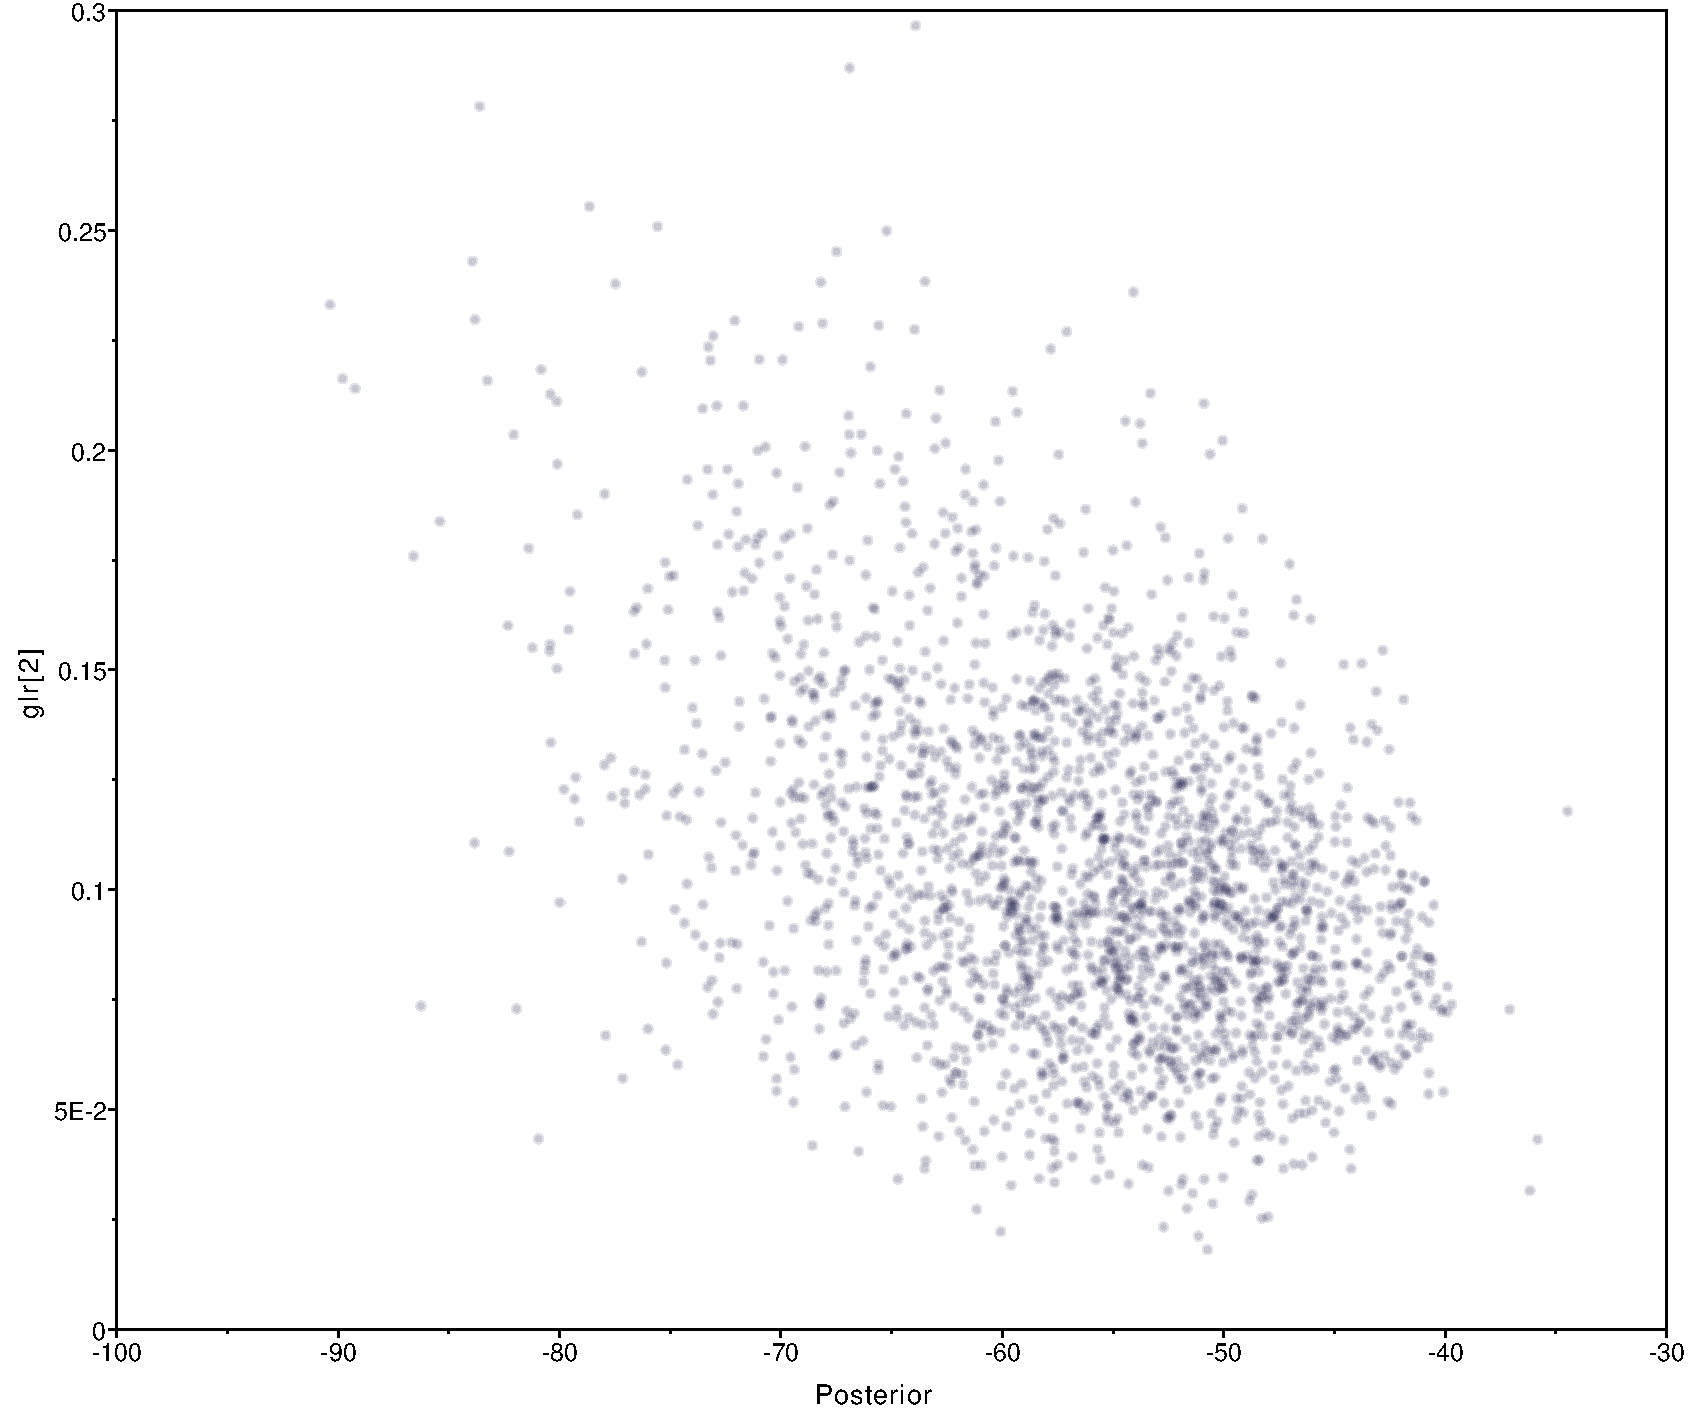
\includegraphics[width=3in]{figures/joint_rgain_posterior}
\end{figure}

Here, we see a strong negative correlation between the posterior probability and the area gain rate, which is expected.

\subsection{Biogeographic event counts from {\tt mnCharHistoryNewick}}

Recording stochastic mappings in a Tracer-compatible format requires some summarization.
This monitor generates a tab-delimited file where the number of events of each type for each branch is recorded.

Open {\tt bg\_2rate.counts.txt}.

\begin{framed}
\begin{lstlisting}[basicstyle=\tiny \listingsfont, columns=texcl]
Iteration	Posterior	Likelihood	Prior	t_s0	t_s1	t_c0	t_c1	t_c2	b0_s0	b0_s1	b0_c	...
0	-60.5999	-60.2078	-0.392113	16	14	37	0	0	1	1	0	...
10	-62.4151	-61.9919	-0.42319	16	14	31	6	0	1	0	1	...
20	-86.6285	-82.9437	-3.68483	26	23	37	0	0	2	2	0	...
30	-49.4231	-50.3783	0.955262	12	12	35	2	0	1	1	0	...
40	-100.982	-95.9841	-4.99809	36	31	35	0	2	1	1	0	...
50	-80.9566	-76.9377	-4.01884	24	23	37	0	0	2	2	0	...
...
\end{lstlisting}
\end{framed}

For example, {\tt b2\_s1} gives the number of areas that are gained for the branch leading to the node indexed 2.
{\tt b2\_c} gives the cladogenic event type that gives rise to the node indexed 2, where sympatry, peripatry, and allopatry are recorded as {\tt 0}, {\tt 1}, and {\tt 2} respectively. The columns {\tt t\_s0} and {\tt t\_s1} give the sum of events over all branches. {\tt t\_c0}, {\tt t\_c1}, and {\tt t\_c2} give the total number of sympatric, peripatric, and allopatric cladogenic events over the entire tree.

Because the expected number of gain events should be proportional to the area gain rate, we expect to see the same negative correlation between posterior probability and number of events as we did with the posterior and rate in the {\tt parameters.txt} file.

Open Tracer, select the fields for the posterior probability and the number of gained areas over the tree, {\tt t1}, then click the Joint-Marginal tab.

\begin{figure}[H]
\centering
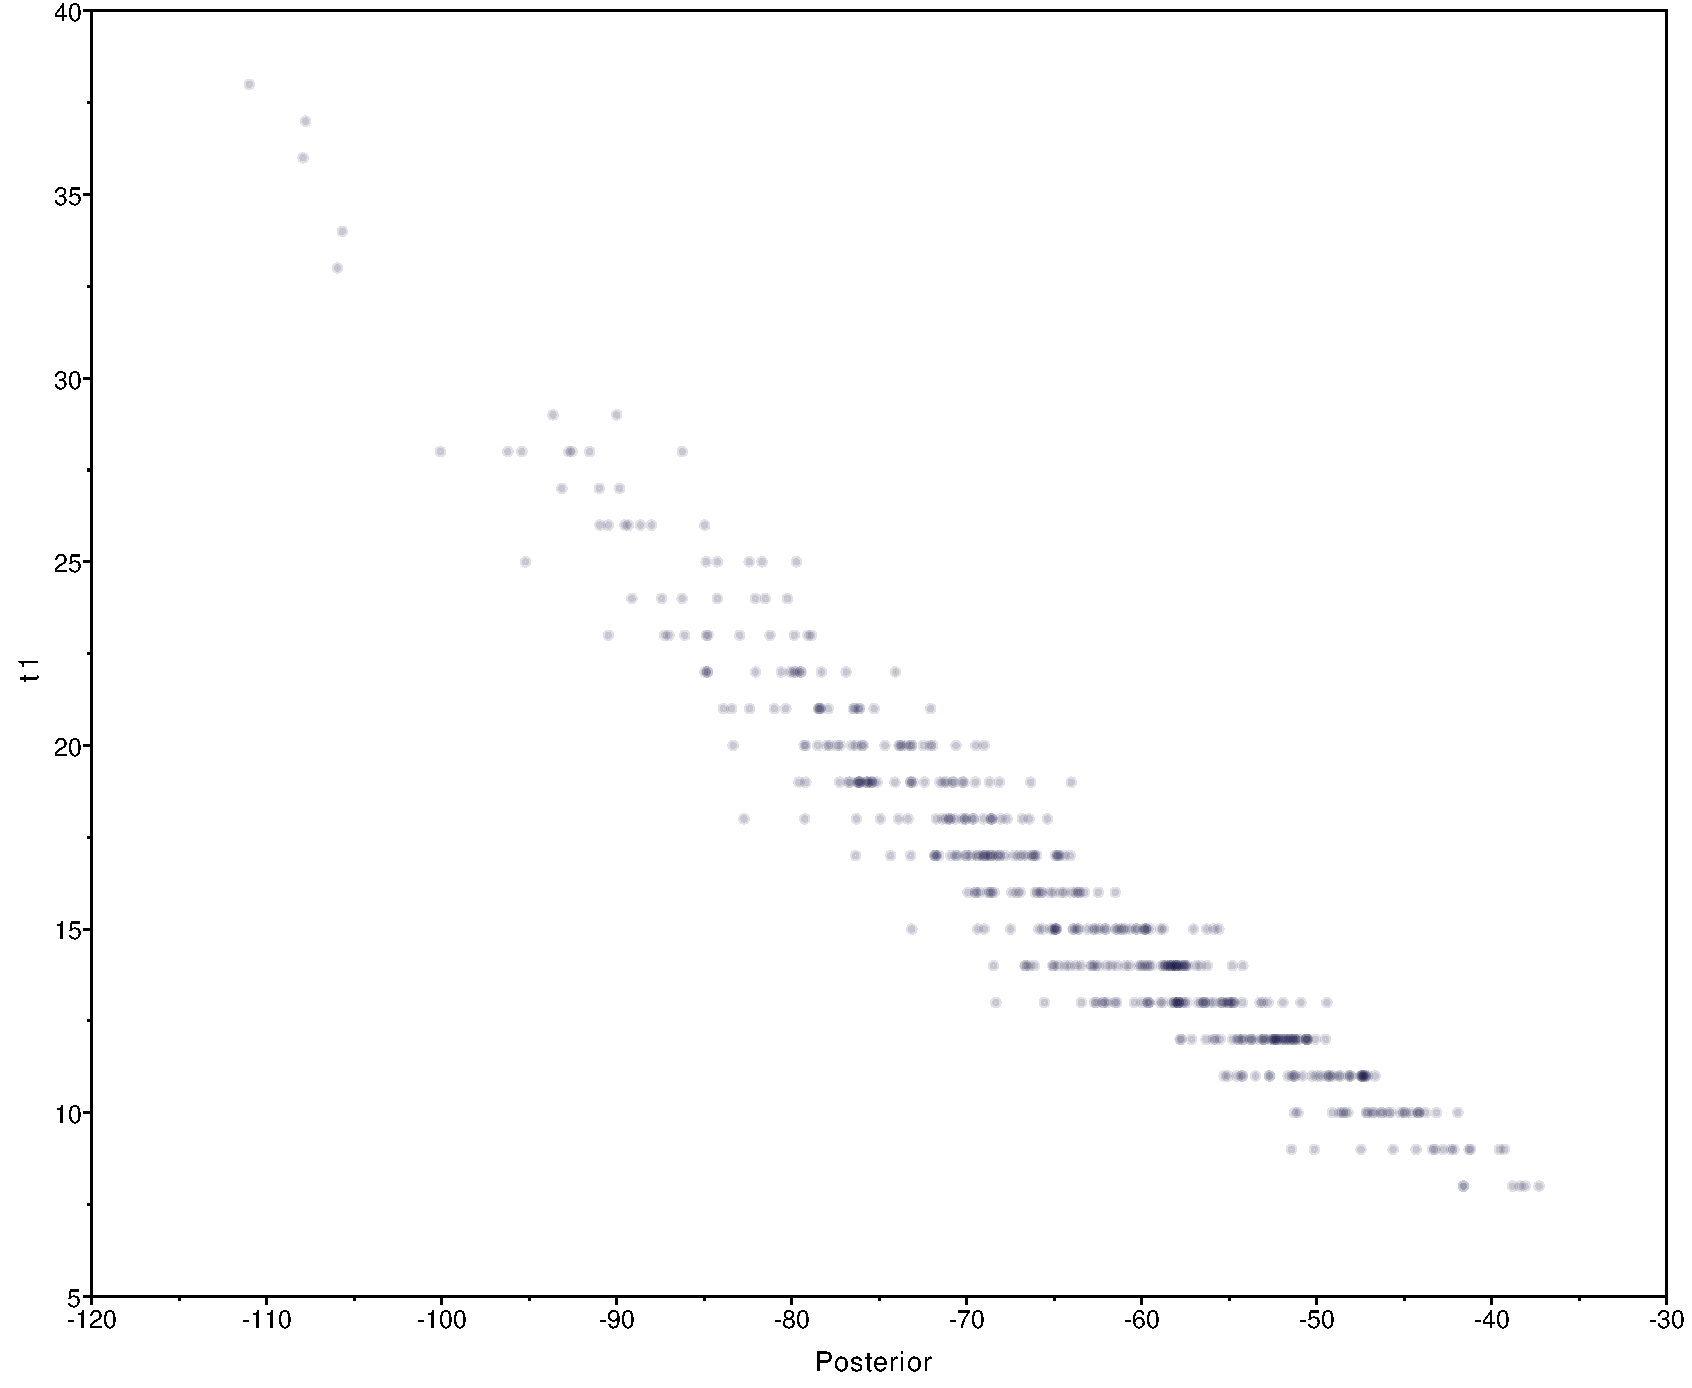
\includegraphics[width=3in]{figures/joint_ngain_posterior}
\end{figure}


\subsection{Biogeographic event histories from {\tt mnCharHistoryNewick}}

For more detailed data exploration, this analysis also provides annotated Newick strings with the complete character mappings for the tree.

Open {\tt bg\_2rate.events.txt}.

\begin{framed}
\begin{lstlisting}[basicstyle=\tiny \listingsfont, columns=texcl]
Iteration	Posterior	Likelihood	Prior	Tree
0	-60.5999	-60.2078	-0.392113	((((((((P_hawaiiensis_WaikamoiL1[&index=18;nd=0010;ev={{t:0.92 ...
10	-62.4151	-61.9919	-0.42319	((((((((P_hawaiiensis_WaikamoiL1[&index=18;nd=0010;ev={{t:0.09 ...
20	-86.6285	-82.9437	-3.68483	((((((((P_hawaiiensis_WaikamoiL1[&index=18;nd=0010;ev={{t:0.30 ...
30	-49.4231	-50.3783	0.955262	((((((((P_hawaiiensis_WaikamoiL1[&index=18;nd=0010;ev={}]:1.08 ...
40	-100.982	-95.9841	-4.99809	((((((((P_hawaiiensis_WaikamoiL1[&index=18;nd=0010;ev={{t:0.16 ...
50	-80.9566	-76.9377	-4.01884	((((((((P_hawaiiensis_WaikamoiL1[&index=18;nd=0010;ev={}]:1.08 ...

...
\end{lstlisting}
\end{framed}

Each iteration records the data-augmented character history (stochastic mapping) using metadata labels, which, for an internal node, looks like

\begin{snugshade}
\begin{lstlisting}
[&index=19;nd=0110;pa=0100;ch0=0010;ch1=0110;cs=p;bn=18;ev={{t:0.139594,a:0.974127,s:1,i:2}}]
\end{lstlisting}
\end{snugshade}

{\tt index=19} indicates this branch leads to the node indexed 19.
The branch began in the ancestral state {\tt pa=0100} and terminated in the state {\tt nd=0110}.
Since this node is not a tip node, it represents a speciation event, so the daughter ranges are also given, {\tt ch0=0010} and {\tt ch1=0110}.
The cladogenic state for this speciation event was peripatric, {\tt cs=p}, rather than sympatric (wide or narrow; {\tt s}) or allopatric ({\tt a}).
Anagenic dispersal and extinction events occurring along the lineage leading to node 19 are recorded in {\tt events}, where each event has a time (relative to the absolute branch length), absolute age, state (into), and character index ({\tt t}, {\tt a}, {\tt s}, {\\t i}, resp.).
For this posterior sample of the character history for the branch leading to node 19, area 2 was gained at age 0.974127, which is near the tips of the tree.

To manipulate this data format, we'll use Python scripts. Below are a few examples of interesting posterior features.

Open a python console and read in the events.

\begin{snugshade}
\begin{lstlisting}
> python27

...

>>> import bg_parse
>>> ll=read_events()
>>> dd=get_events(ll)
\end{lstlisting}
\end{snugshade}


Each branch is a dictionary whose keys are various parts of the MCMC state and whose values the MCMC samples.
\begin{snugshade}
\begin{lstlisting}
>>> dd[19].keys()
['ch1', 'iteration', 'bn', 'nd', 'ch0', 'prior', 'posterior', 'cs', 'ev', 'likelihood']
>>> dd[19]['posterior'][0:5]
[-60.5999, -62.4151, -86.6285, -49.4231, -100.982]
>>> dd[19]['cs'][0:5]
['s', 'p', 's', 's', 's']
\end{lstlisting}
\end{snugshade}

To get the $n=1$ highest-valued sample for a branch by its posterior value
\begin{snugshade}
\begin{lstlisting}
>>> get_best(dd[19],n=1,p='posterior')
{'prior': [2.25647], 'iteration': [940], 'bn': [18], 'nd': [[0, 0, 1, 0]], 'ch0': [[0, 0, 1, 0]], 'ch1': [[0, 0, 1, 0]], 'posterior': [-36.9044], 'cs': ['s'], 'ev': [[{'age': 0.705193, 'state': 1, 'idx': 2, 'time': 0.477281}, {'age': 0.607798, 'state': 0, 'idx': 1, 'time': 0.599575}]], 'likelihood': [-39.1609]}
\end{lstlisting}
\end{snugshade}

To get the probability that area $i$ and area $j$ are both part of the species range as the branch for node 19 terminates, just before the speciation event
\begin{snugshade}
\begin{lstlisting}
>>> get_area_pair(dd[19],k='nd')
[[0.07892107892107893, 0.014985014985014986, 0.06793206793206794, 0.0],
[0.014985014985014986, 0.3956043956043956, 0.3546453546453546, 0.0],
[0.06793206793206794, 0.3546453546453546, 0.952047952047952, 0.0],
[0.0, 0.0, 0.0, 0.0]]
\end{lstlisting}
\end{snugshade}
showing area 3 was occupied with probability 0.95 and both areas 2 and 3 were occupied with probability 0.35.

If the range is size one during a speciation event, the cladogenic event state is always sympatric, ``s''.
But given the opportunity for non-sympatric events, i.e. that the range is larger than size one, we can get the probability of cladogenic state using
For the probability for cladogenic event state given the range was larger than size one
\begin{snugshade}
\begin{lstlisting}
>>> get_clado_state(dd[19],minSize=1)
{'a': 0.027972027972027972, 'p': 0.2037962037962038, 's': 0.7682317682317682}
>>> get_clado_state(dd[19],minSize=2)
{'a': 0.0673076923076923, 'p': 0.49038461538461536, 's': 0.4423076923076923}
\end{lstlisting}
\end{snugshade}

For more examples, see {\tt bg\_parse.py}

\subsection{New Hampshire extended format file (\texttt{my\_run.nhx})}

Because this data is very high-dimensional, we'll use an external data exploration tool to look at range evolution.

This file summarizes the input and output from a BayArea analysis using NEXUS format containing a New Hampshire eXtended (NHX) tree string.
NHX allows you to annotate nodes in a Newick string with meta-information, which BayArea uses to report the probabilities in the \texttt{my\_run.area\_probs.txt} file.
The \texttt{geo} block gives the geographical latitudes and longitudes for the areas in the order they are reported as probabilities.
Like the \texttt{my\_run.area\_probs.txt} file, this file is not written until the analysis is complete.
This annotation is used for the two visualization programs covered in the next section, Phylowood and BayArea-Fig.
The anatomy of the Phylowood and BayArea-Fig settings blocks will also be explained there.

\section{Visualization}

Here we'll explore two options for visualizing ancestral range reconstructions.
I'll walk you through some of the basic functionality, but feel free to play around as you like.

\subsection{Phylowood}

Phylowood generates interactive animations to explore biogeographic reconstructions.

\noindent \\ \impmark Open \texttt{http://mlandis.github.io/phylowood}.

\noindent \\ \impmark Drag and drop \texttt{bg\_2rate.nhx.txt} into the text field.

\begin{figure}[H]
\centering
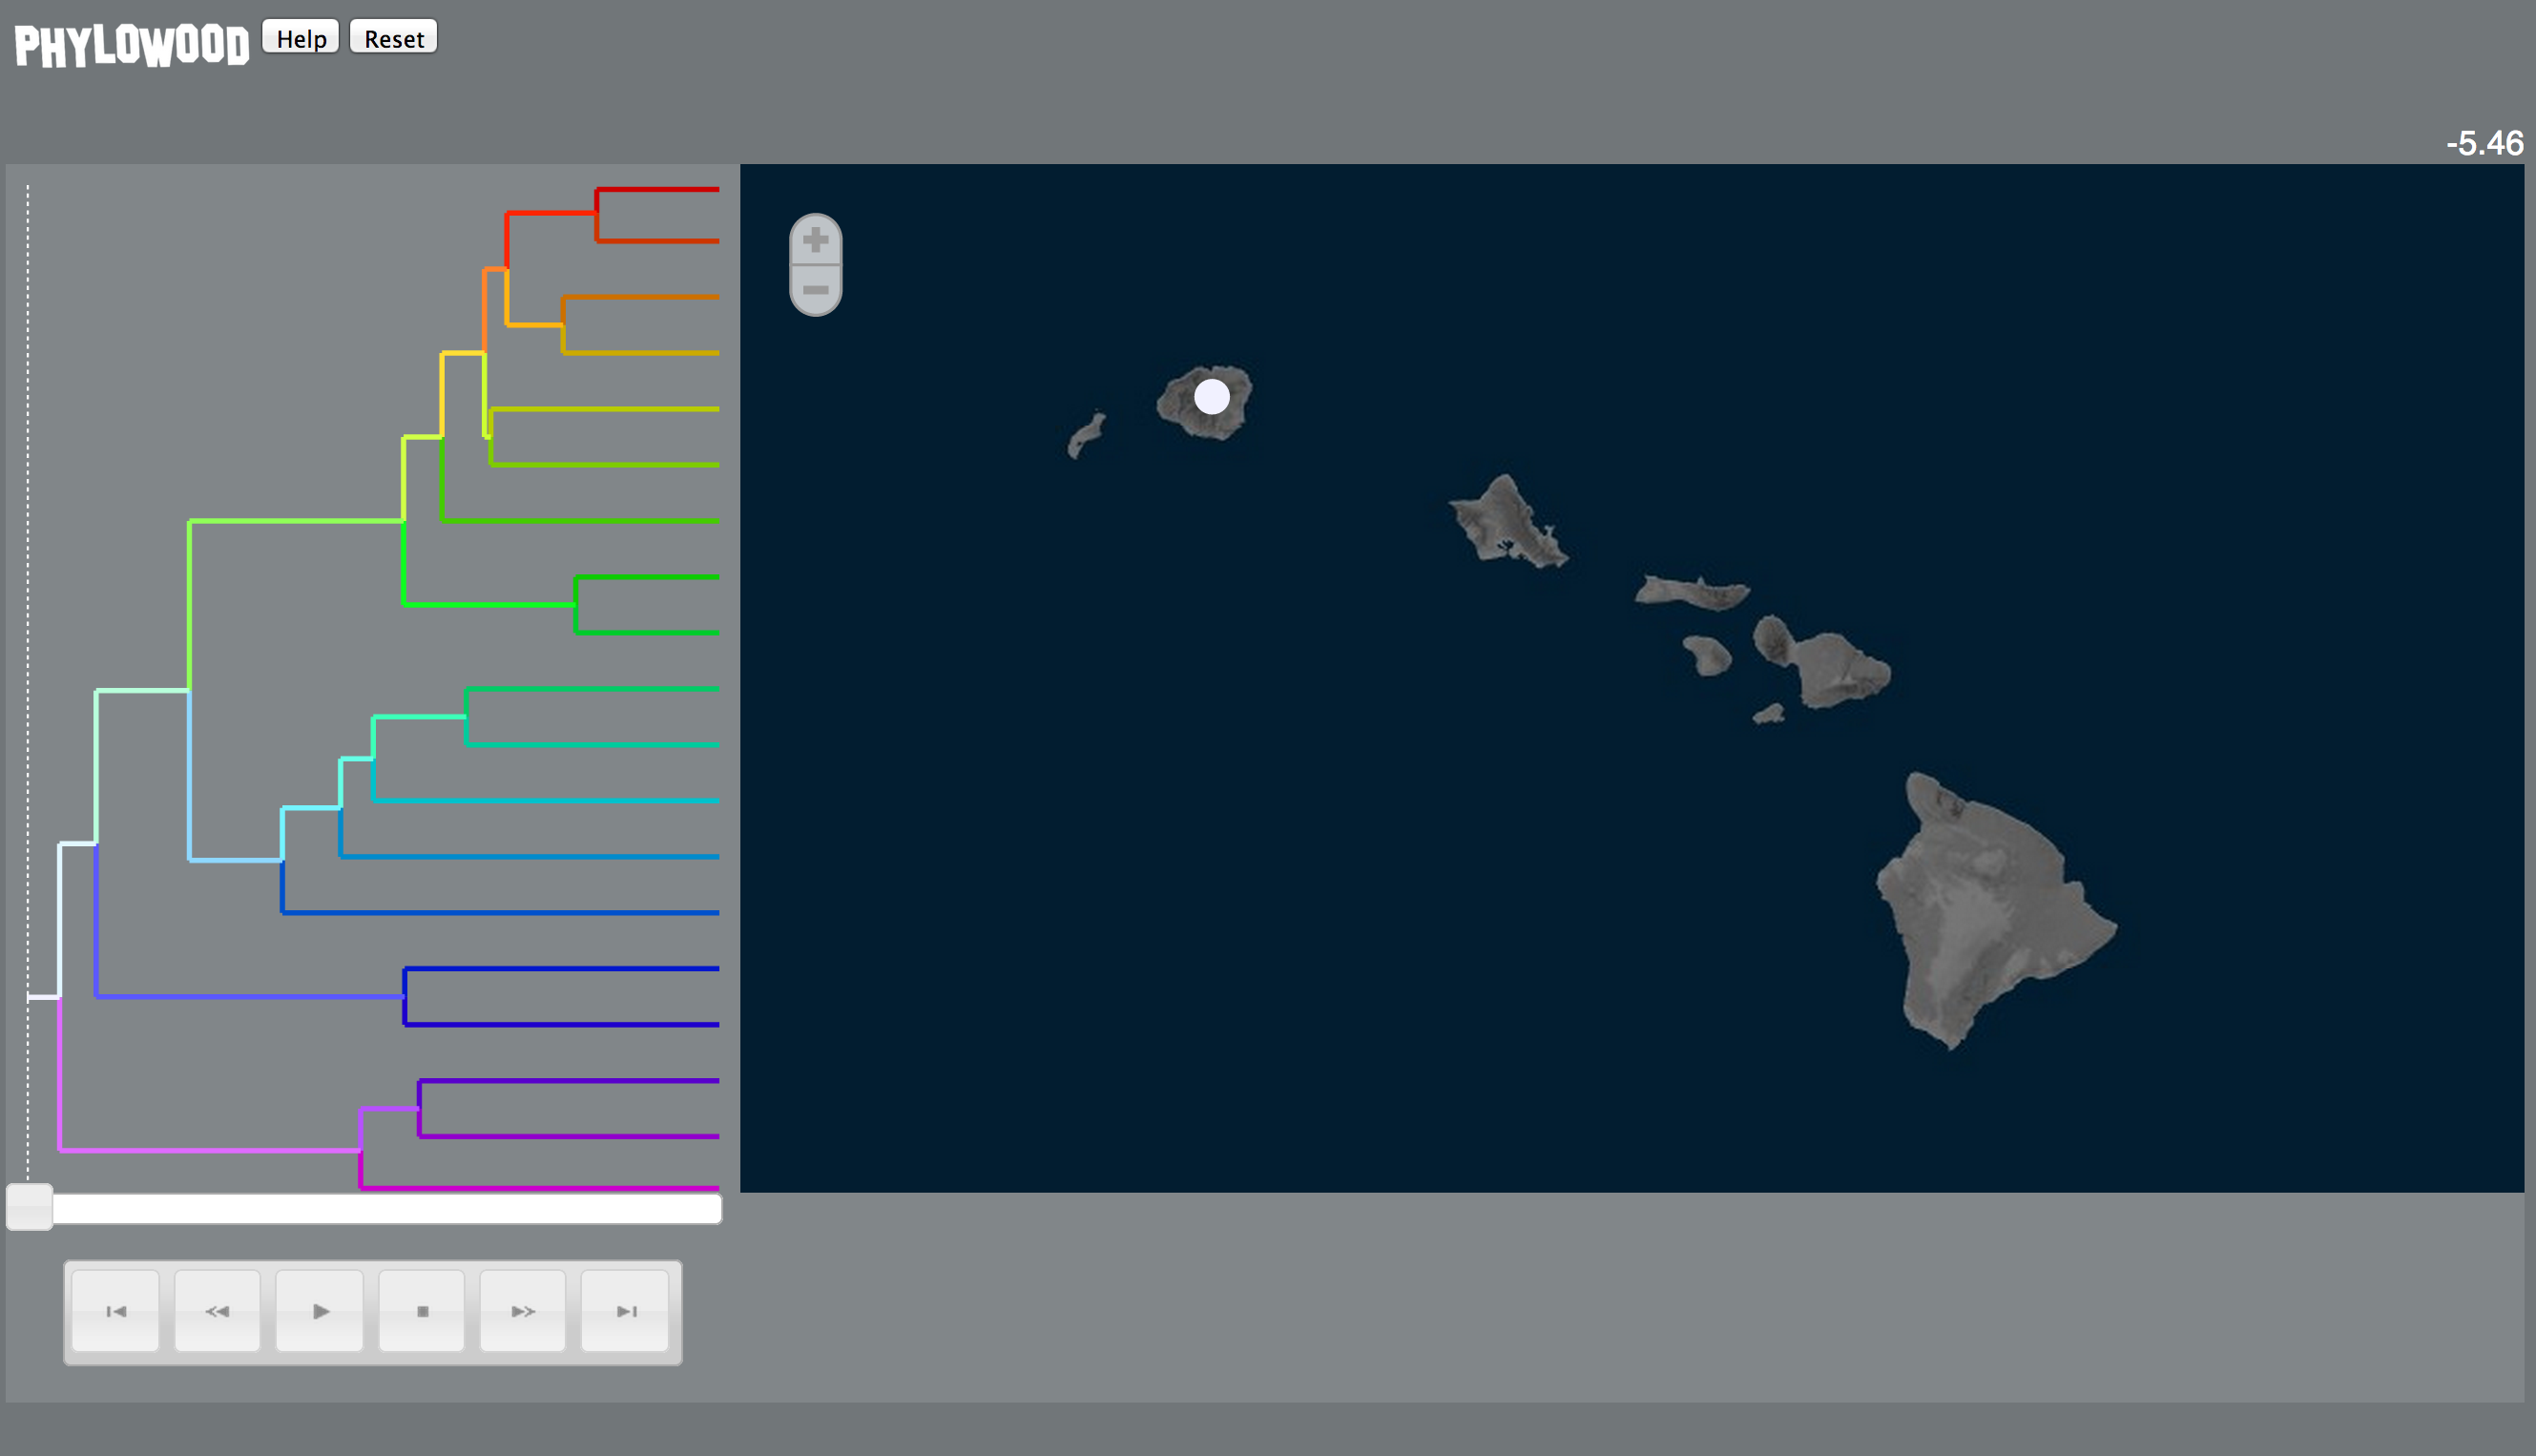
\includegraphics[width=4in]{figures/phw_mrca}
\end{figure}

\noindent \\ \impmark Click the Play button to view the animation. \\

There are three control panels to help you filter data: the media panel, the map panel, and the phylogeny panel.
The media buttons correspond to Beginning, Slow/Rewind, Play, Stop, Fast Forward, Ending (from left to right).
The animation will play the timeframe corresponding to the slider.

\noindent \\ \impmark Drag the slider to the right (the present).

\begin{figure}[H]
\centering
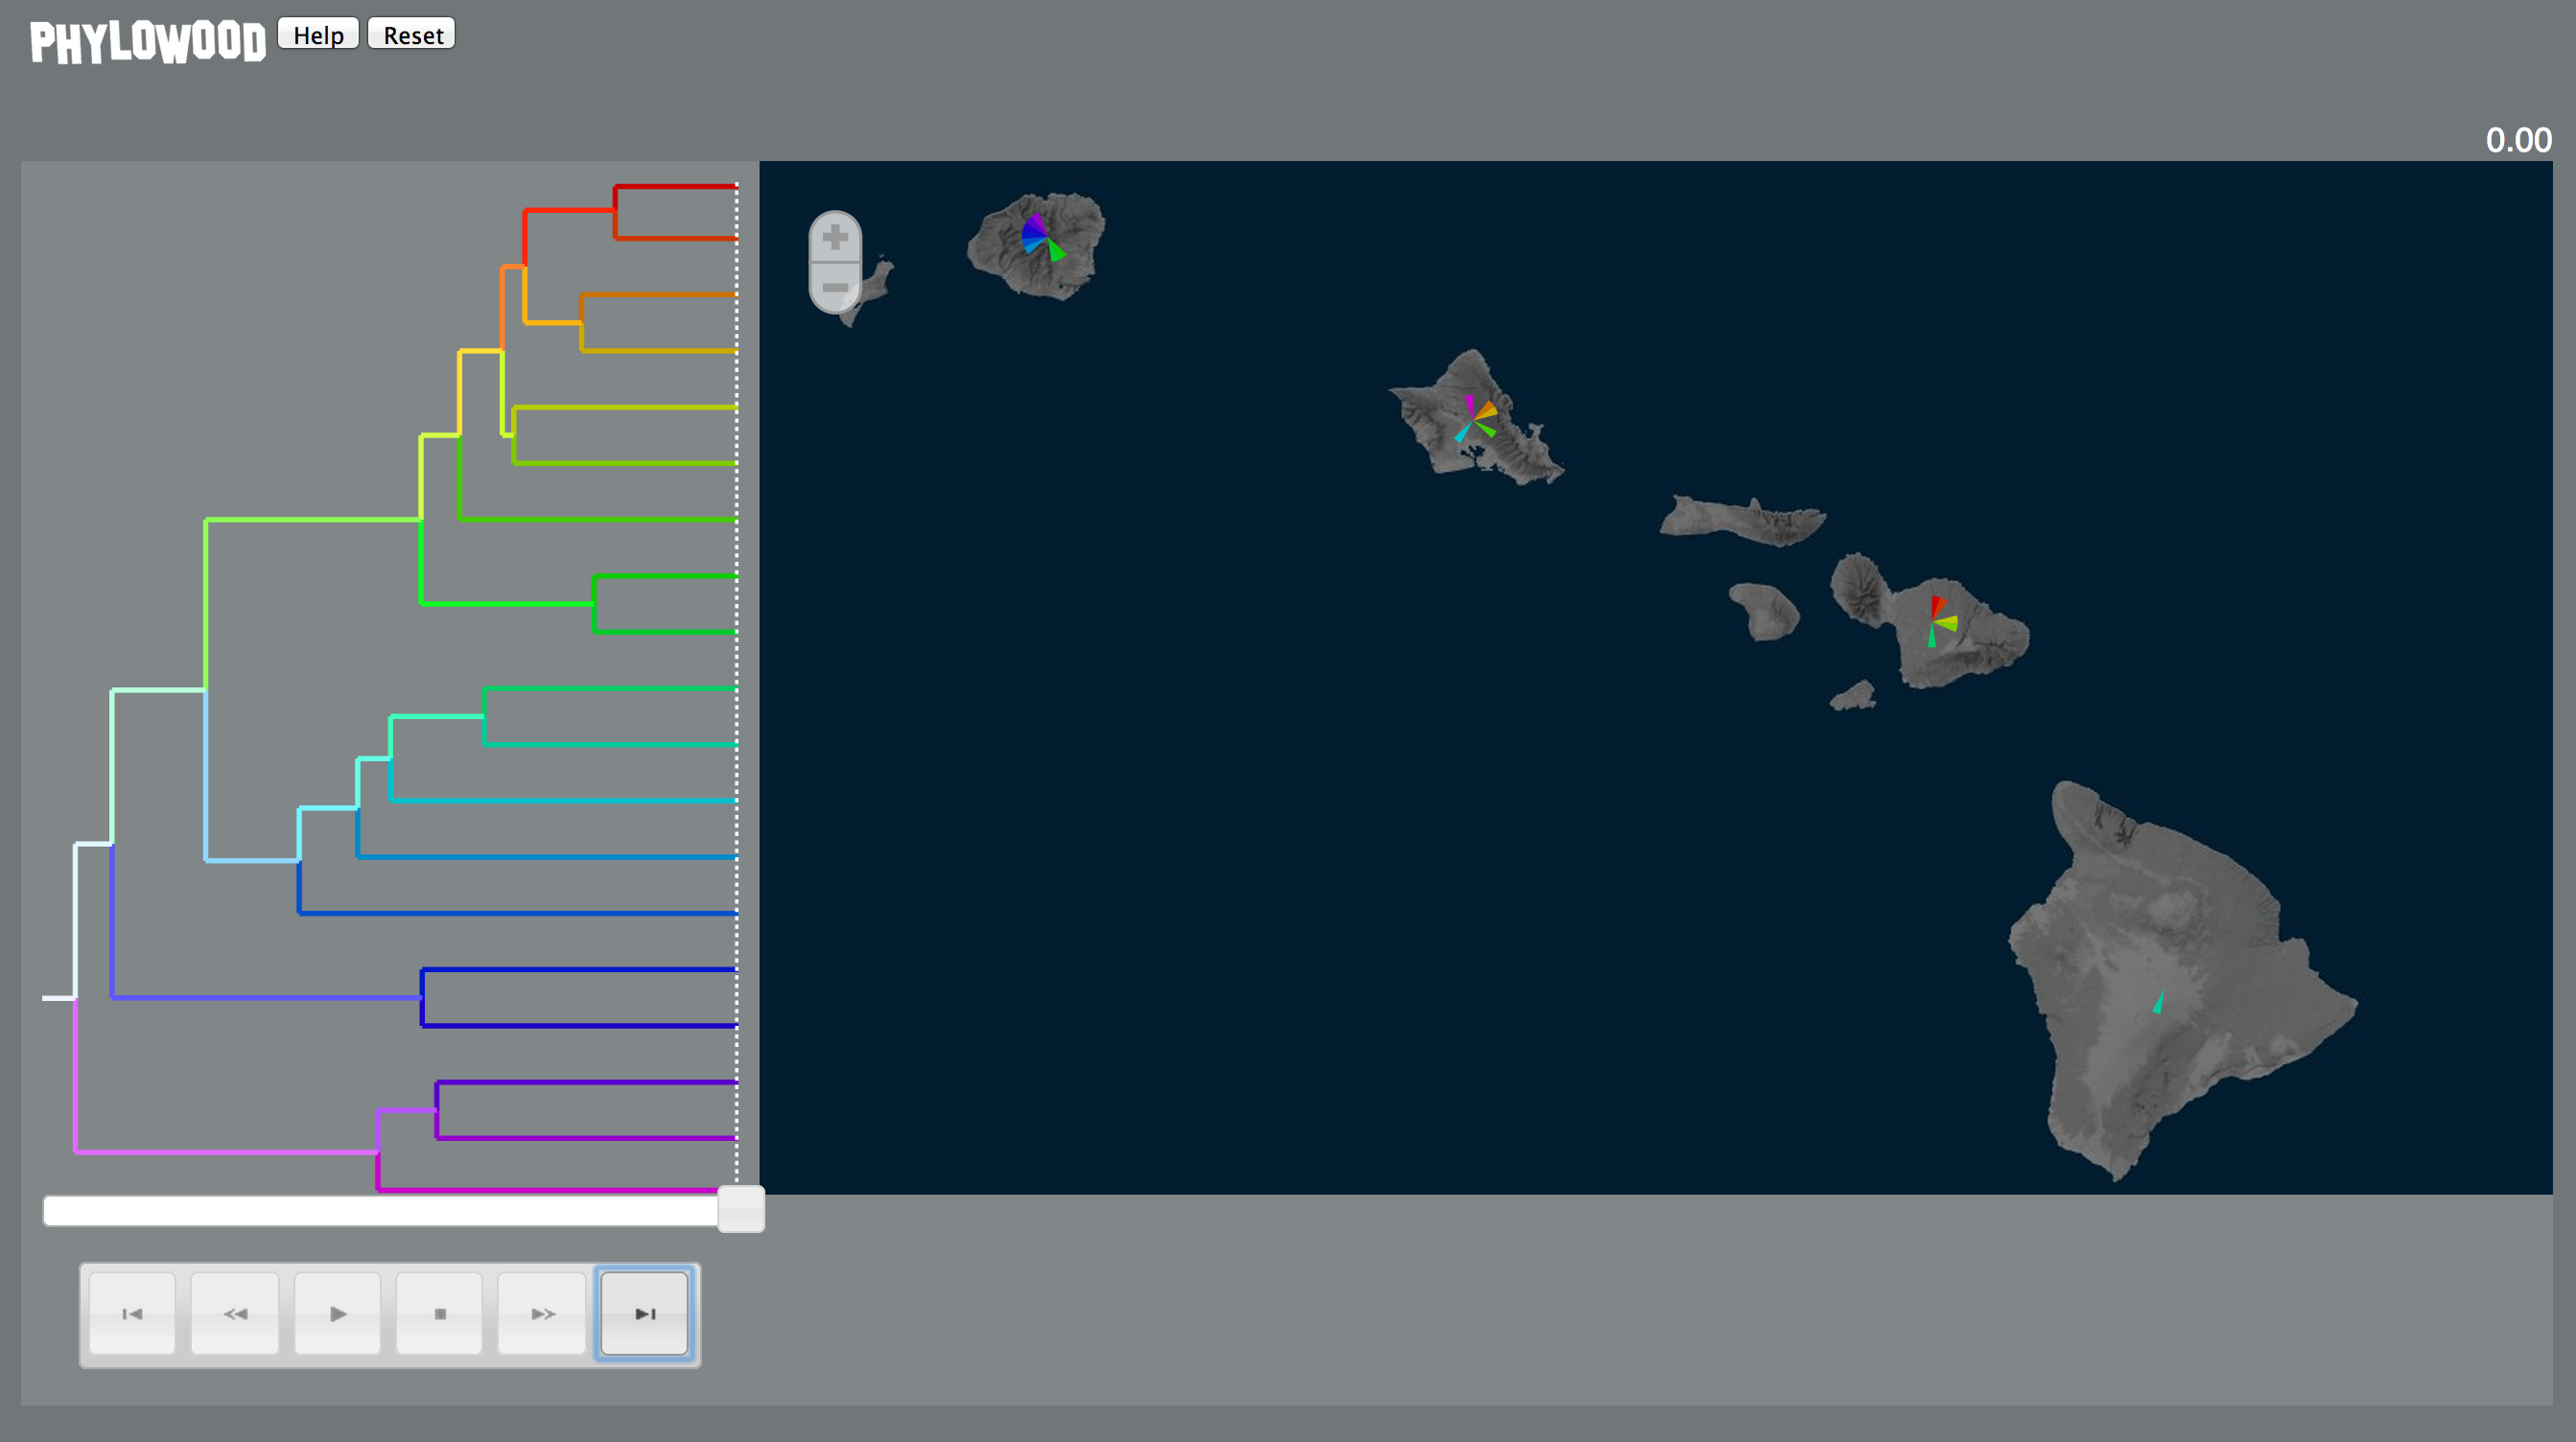
\includegraphics[width=4in]{figures/phw_all}
\end{figure}

\noindent \\ \impmark Pan and zoom around the map.\\

Marker colors correspond to the phylogenetic lineages in the phylogeny panel.
Markers are split into slices and (loosely) sorted phylogenetically, so nearby slices are generally closely related.
At divergence events, a marker's radius is proportional to the marginal posterior probability the node was present in the area at that time.
Between divergence events, marker's radius is simply an interpolation of the values at the two endpoints.
Some information about geological constraints and cladogenic events is lost.

\noindent \\ \impmark Mouseover an area to learn which lineage it belongs to and its presence probability. \\

Since it's difficult to see how specific clades evolve with so many taxa, Phylowood offers two ways to filter taxa from the animation.
We call the set of a lineage, all its ancestral lineages towards the root, and all descendant lineages a phylogenetic heritage.
The root's heritage is the entire clade.
A leaf node's heritage is a path from the tip to the root.

\noindent \\ \impmark Mouseover a lineage to temporarily highlight the lineage's heritage. Remove the mouseover to remove the highlight effect. \\

The highlight effect is temporary and quickly allows you to single out lineages of interest during animation.
Phylowood also offers a masking effect that persists until an unmask command is issued.

\noindent \\ \impmark Double-click the white root branch to mask the root node's heritage (all lineages). Single click a lineage to unmask that lineage's heritage. \\

\begin{figure}[H]
\centering
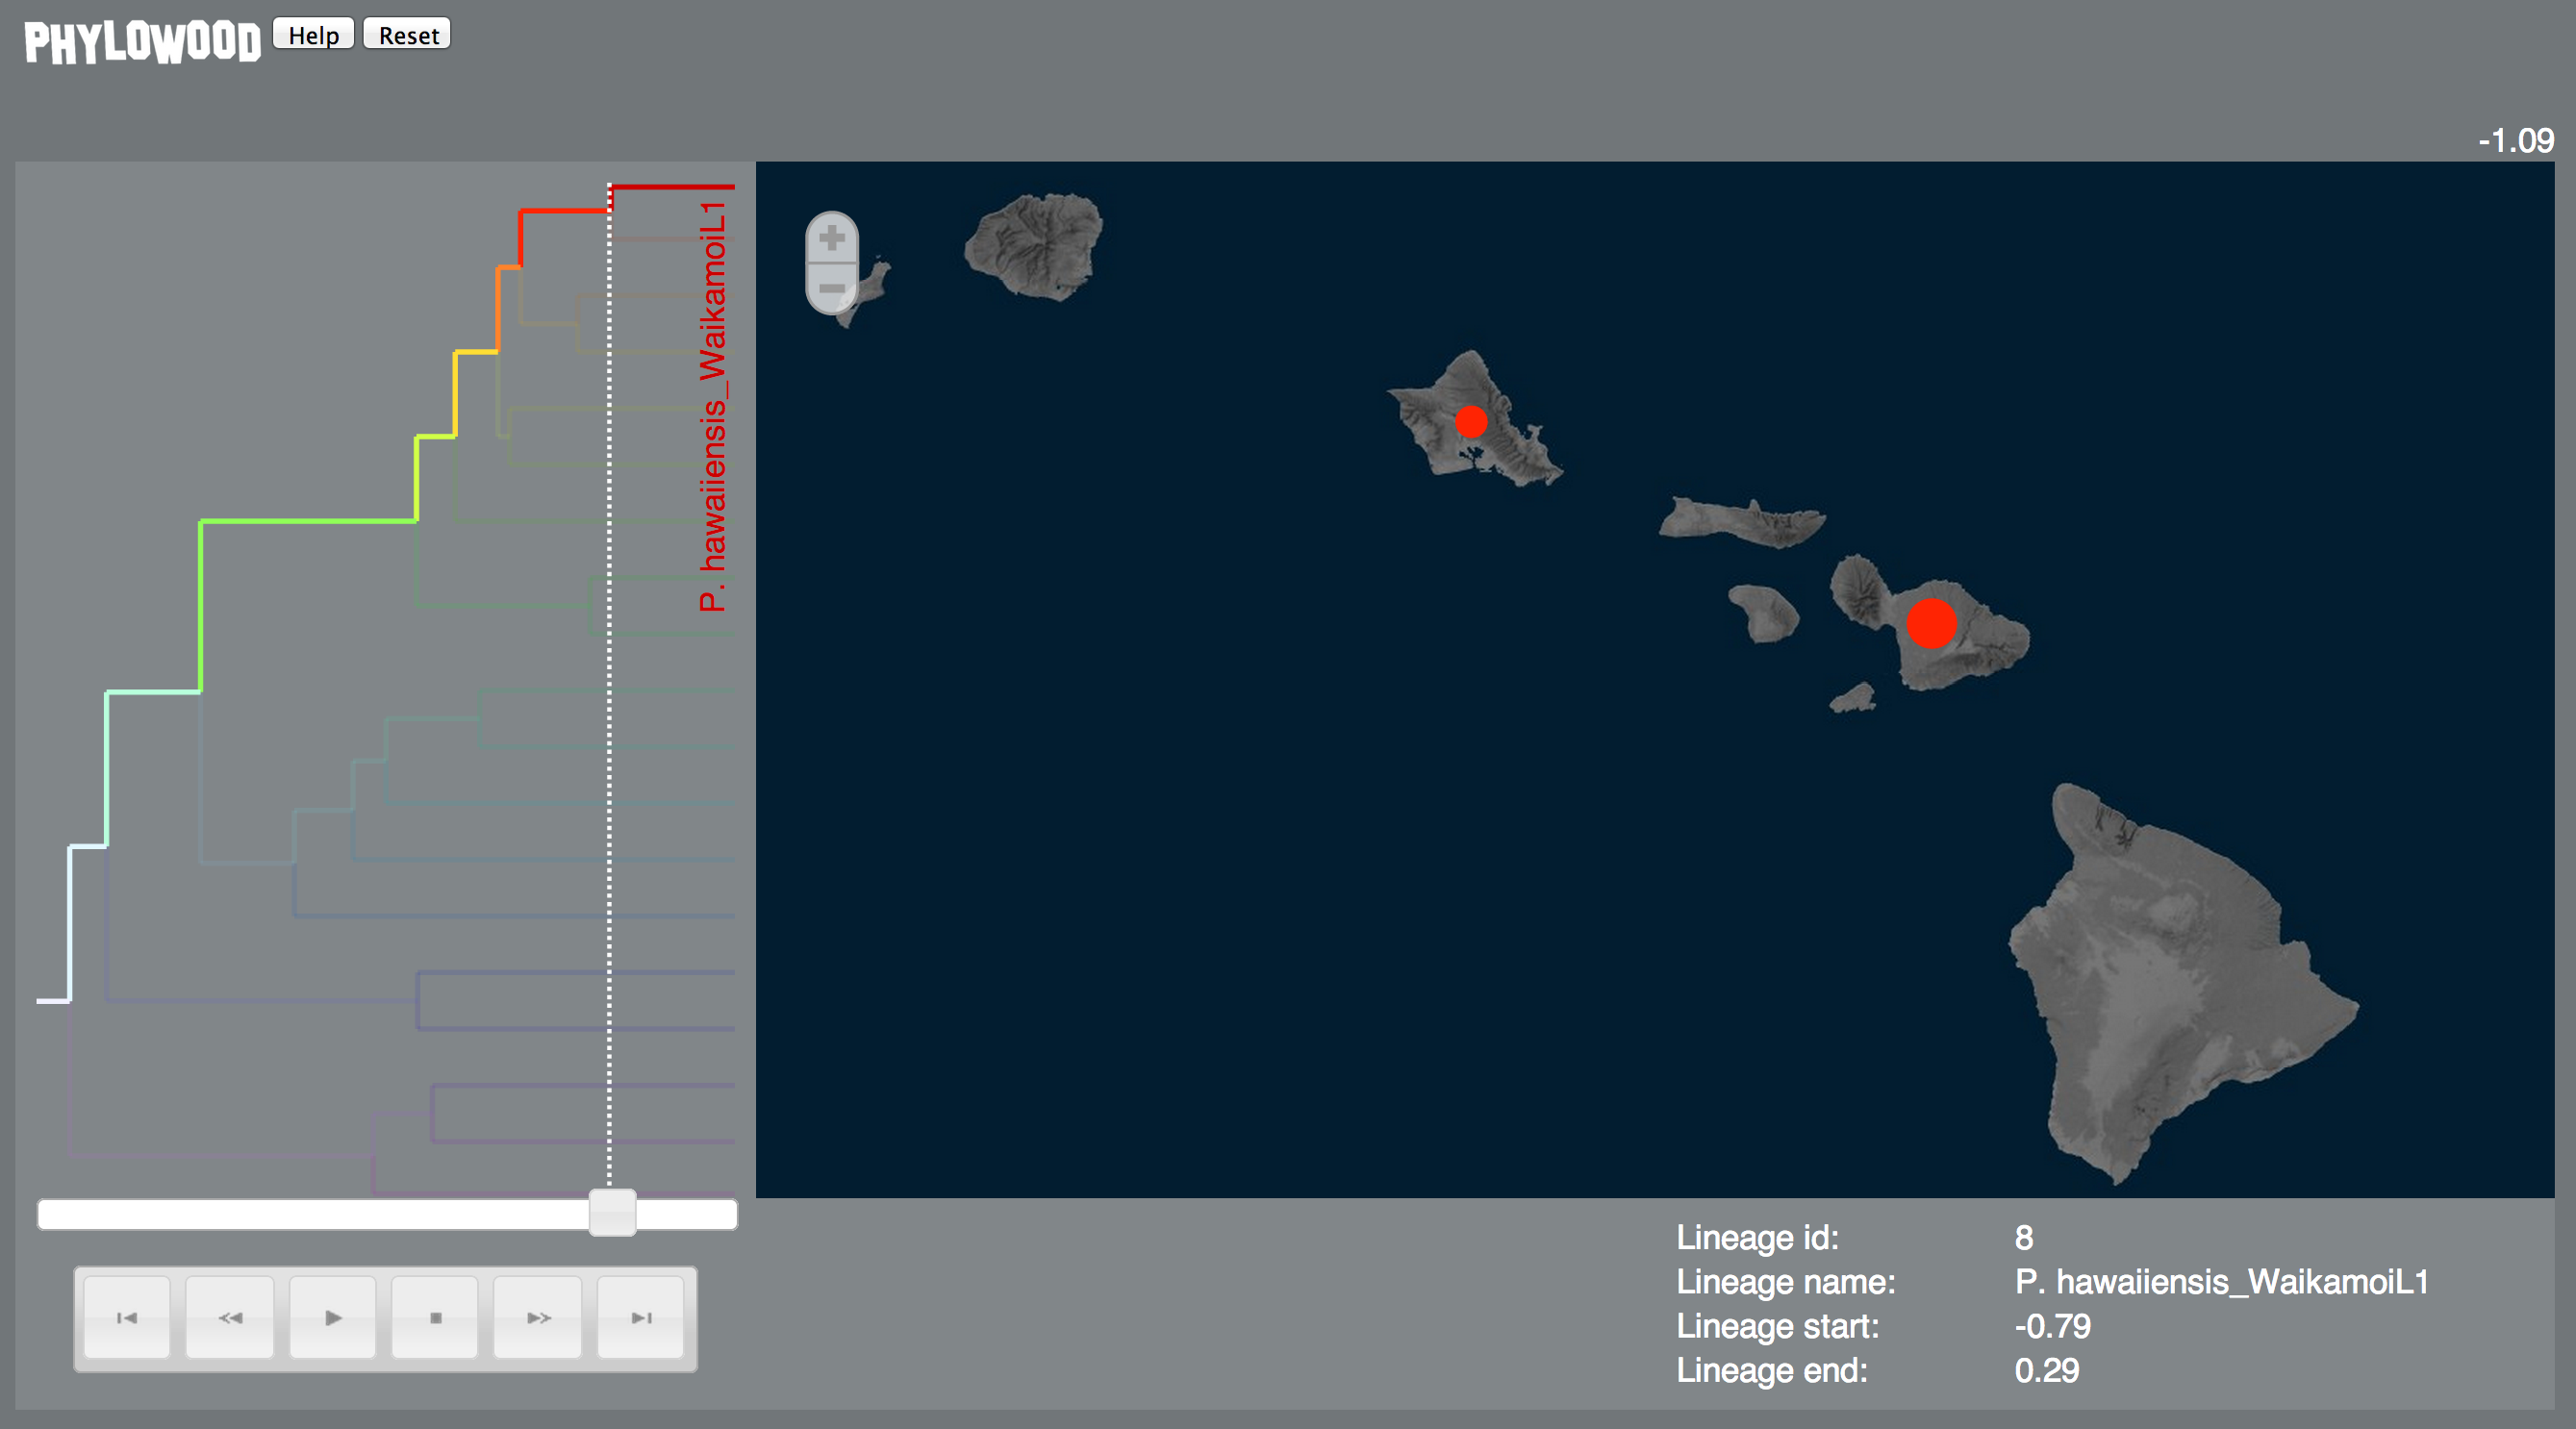
\includegraphics[width=4in]{figures/phw_br19}
\end{figure}

Now that the masking effects are in place, you're free to interact with other map components.
In addition, the area of marker sizes is only distributed among unmasked lineages.

\noindent \\ \impmark Visit \texttt{https://github.com/mlandis/phylowood/wiki} to learn more about Phylowood.

%
%\subsection{BayArea-Fig}
%
%BayArea-Fig is a simple Javascript utility to help generate ancestral range reconstruction figures for publications.
%BayArea 1.0.2 does not automatically generate the NEXUS settings block for BayArea-Fig, so I added the following block to \texttt{my\_run.nhx}.
%
%%\noindent \\ \impmark  Add the following code after the \texttt{\#NEXUS} header in \texttt{my\_run.nhx} and save the file.
%\begin{framed}
%\begin{lstlisting}
%Begin bayarea-fig;
%	mapheight 100
%	mapwidth 150
%	canvasheight 2000
%	canvaswidth 2000
%	minareaval 0.1
%	areacolors blue red
%	areatypes 0 1 0 0 0 1 1 0 0 0 0 1 1 1 0 0 0 0 1 1 1 1 0 0 0 0 1 1 1 1 1 1 1
%	areanames West East
%End;
%\end{lstlisting}
%\end{framed}
%
%\noindent \\ \impmark  Open \texttt{http://mlandis.github.io/bayarea-fig} in a web browser.
%
%\noindent \\ \impmark  Drag and drop \texttt{my\_run.nhx} into the text field. \\
%
%\begin{figure}[H]
%\centering
%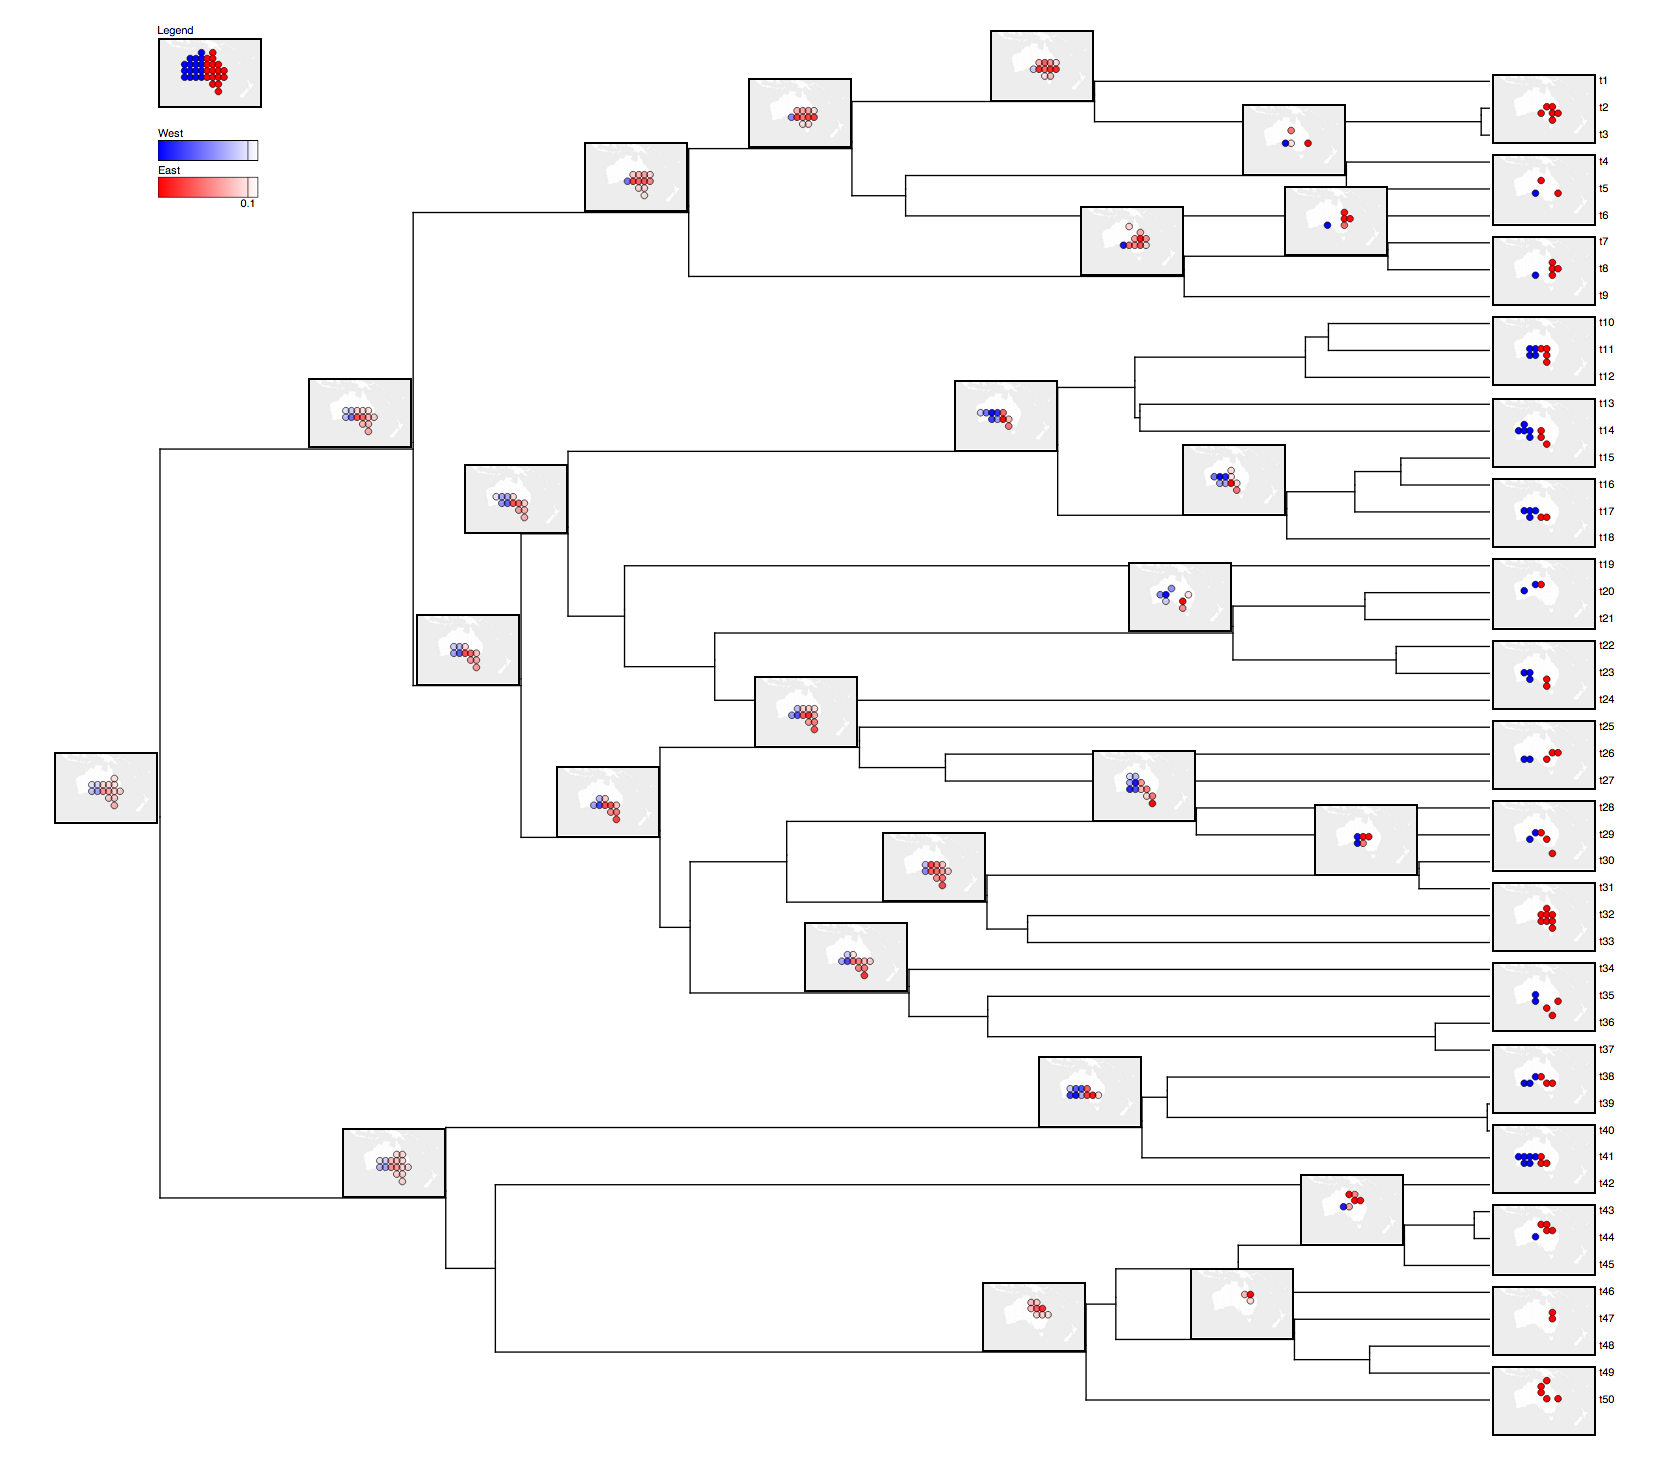
\includegraphics[width=4in]{figures/bayarea-fig}
%\end{figure}
%
%The generated figure reports the marginal area probabilities for each node in the phylogeny with a miniature map.
%Because of the limited real estate in the figure, you may only wish to show a subset of ancestral ranges.
%
%\noindent \\ \impmark  Click unwanted ancestral ranges to delete them. \\
%
%Depending on the purpose for the figure, you may wish to alter its size.
%The \texttt{mapheight}, \texttt{mapwidth}, \texttt{canvasheight}, and \texttt{canvaswidth} settings give the height and widths for the node-maps and the entire figure, respectively.
%
%If you would like to differentiate areas (e.g. East from West, as above), give an ordered list of colors using the \texttt{areacolors} setting.
%Next, in the order areas appear in the $\texttt{GEO}$ block, provide \texttt{areatypes} a list of assigments to area types.
%In the above example ``0'' corresponds to the 0th \texttt{areacolors} group, ``blue'', and ``1'' corresponds to the 1st group, ``red''.
%
%\noindent \\ \impmark Add a new color as the third \texttt{areacolors} entry. Add ``Tasmania'' as a third entry to \texttt{areanames}. Change the last area in \texttt{areatypes} to equal 2. \\
%
%We've seen that ancestral range reconstructions contain a great deal of uncertainty.
%Filtering out low probability ranges may make your figure easier to interpret.
%If the marginal probability of presence for a node-area pair is less than \texttt{minareaval}, it is not shown.
%The probabilities and the threshold value are shown in the upper left corner.
%
%After arranging your figure, you'll want to save it to file.
%How to accomplish this varies across operating systems and web browsers.
%Generally, the figure is most easily saved from the browser by printing the file to pdf.
%In this case the image size is equal to the paper size.
%If the standard $8.5 \times 11$ inch image is too small, you will need to create and apply a sufficiently large custom paper size.

\bibliography{bayes}

%\newpage
%\begin{sidewaysfigure}
%\centering
%\includegraphics[width=9in]{figures/bg_mol_dag}
%\caption{Joint inference of range and molecular data. This figure explodes the module components in Figure \ref{fig:bm_mod}}
%\label{fig:bm_dag}
%\end{sidewaysfigure}

\end{document}


% old stuff


%{\it If you want to construct your own data matrix, I'll go over these topics below: collecting species occurrence data, identifying the total geographic region to include for analysis, and discretizing the geography into areas.}
%
%\subsubsection{Collecting species occurrence data}
%
%Species occurrence data minimally reports the latitude and longitude of a species of interest.
%For our analysis, a species is present in an area so long as that area contains a single occurrence record.
%For large areas, presence-absence characters are fairly robust to small measurement errors in geographical coordinates or imperfect sampling.
%[ I expect taxon sampling to be rel. unbiased since all biodiversity recorded per ``area''. ]
%I recommend querying the Global Biodiversity Information Facility (GBIF) database for a preliminary species occurrence dataset.
%
%[ Query georeference data ]
%Steps...
%
%[ Note gross outliers ]
%Some occurrence data may refer to museum or zoo specimens, or may be entirely erroneous (e.g. set to the default (latitude, longitude) of (0$^\circ$,0$^\circ$).
%
%[ Download data ]
%
%The default GBIF species occurrence query results are stored in the tab-delimited file, occurrence.txt.
%Using your favorite scripting language, you can easily extract the list of geographical coordinates per species.
%Because species names vary slightly between GBIF submissions, you should also take care to combine mismatched entries.
%Here is an example of the extracted (and cleaned) species occurrence data contained in occurrence.txt.
%
%\begin{framed}
%\begin{lstlisting}
%Canis lupus	-23.57222	132.78139
%Canis lupus	-13.75433	136.85133
%Canis aureus	33.06980	35.28452
%Canis aureus	32.02343	35.51647
%Canis latrans	45.89355	-69.99026
%...
%\end{lstlisting}
%\end{framed}
%
%Species with few or no GBIF occurrence records should be considered suspicious and supplemented with occurrence data reported in the scientific literature or (if applicable) taxon-specific biodiversity databases.
%
%So your work is useful, wait until after constructing the presence-absence data matrix to assess whether additional species occurrence records are required.
%
%\subsubsection{Identifying the total geographic region}
%
%Here we'd like to identify the geographic region(s) on Earth that extant and ancestral taxa may have occupied.
%For example, if you are studying purely terrestrial species, you may wish to exclude regions that contain no land.
%These regions will later be discretized into areas, then assigned presence-absence range data from the species occurrence records.
%The region(s) should minimally envelope all species occurrence data.
%
%[ Image ]
%
%You should consider two things before choosing to exclude certain regions from the analysis.
%First, is the region intermediate to the ranges of extant taxa?
%For instance, if sister taxa are endemic to North and South America respectively, then Central America may be considered for omission.
%However, this would forbid ancestral ranges from passing through the omitted region and greatly affect inference.
%Second, is the region 
%The range evolution model assumes a taxon is extinct when it is absent in all areas in the analysis.
%Extinction is always correctly considered when the set of areas covers the entire globe.
%
%\subsubsection{Discretizing the geography into areas}
%
%Geographic space is inherently continuous, so discretizing the geography into areas is a somewhat arbitrary process.
%Not much research has been done exploring how to best declare areas, so this section will introduce various strategies you may wish to consider.
%
%[ Image ]
%
%{\it Natural discretization.}
%Some regions are clearly discretized into areas, such as island archipelagos.
%Other regions contain suggested areas, such as those delimited by mountain ranges and bodies of water.
%Dispersal barriers will depend on the life history traits of your study taxa.
%Marking islands with presence-absence characters is quite easy while determining whether a point is within a polygon on the surface of a sphere is a more challenging problem in geometry.
%
%{\it Published discretization.}
%Biogeographic methods have defined areas in a variety of ways, using area cladograms, areas of endemism, etc.
%It may be tempting to use areas from previous biogeographic analyses for a BayArea (or other) statistical biogeographic analysis, but be wary.
%For instance, if parsimony-uninformative areas are discarded, then the inference of range expansion and contraction rates will surely be affected, which directly affects the ancestral range reconstructions.
%
%{\it Uniform discretization.}
%If you are unable to apply a satisfying rationale to define your areas, you could apply a uniform discretization over the geography.
%This strategy will treat the Earth as a sphere then discretize it using geodesic tiling (equilateral triangles).
%In this approach, all areas are equal in size and shape.
%The symmetry of uniform discretization offers some aid to easily identify which species are present in which areas.
%The following Python script generates a geodesic tiling, excludes water (or land) areas, converts species occurrence data into presence-absence characters, and writes files for the data matrix and area coordinates (below).


%
%Open the \texttt{my\_run.parameters.txt} in Tracer.
%First, we see the effective sample size is only moderate for $50 \times 10^6$ cycles when sampling every 1000 cycles.
%This is because the vast majority of MCMC updates are range history updates.
%
%\noindent \\ \impmark  Highlight the ``gain'' and ``loss'' parameters then click Joint-Marginal.
%
%\begin{figure}[H]
%\centering
%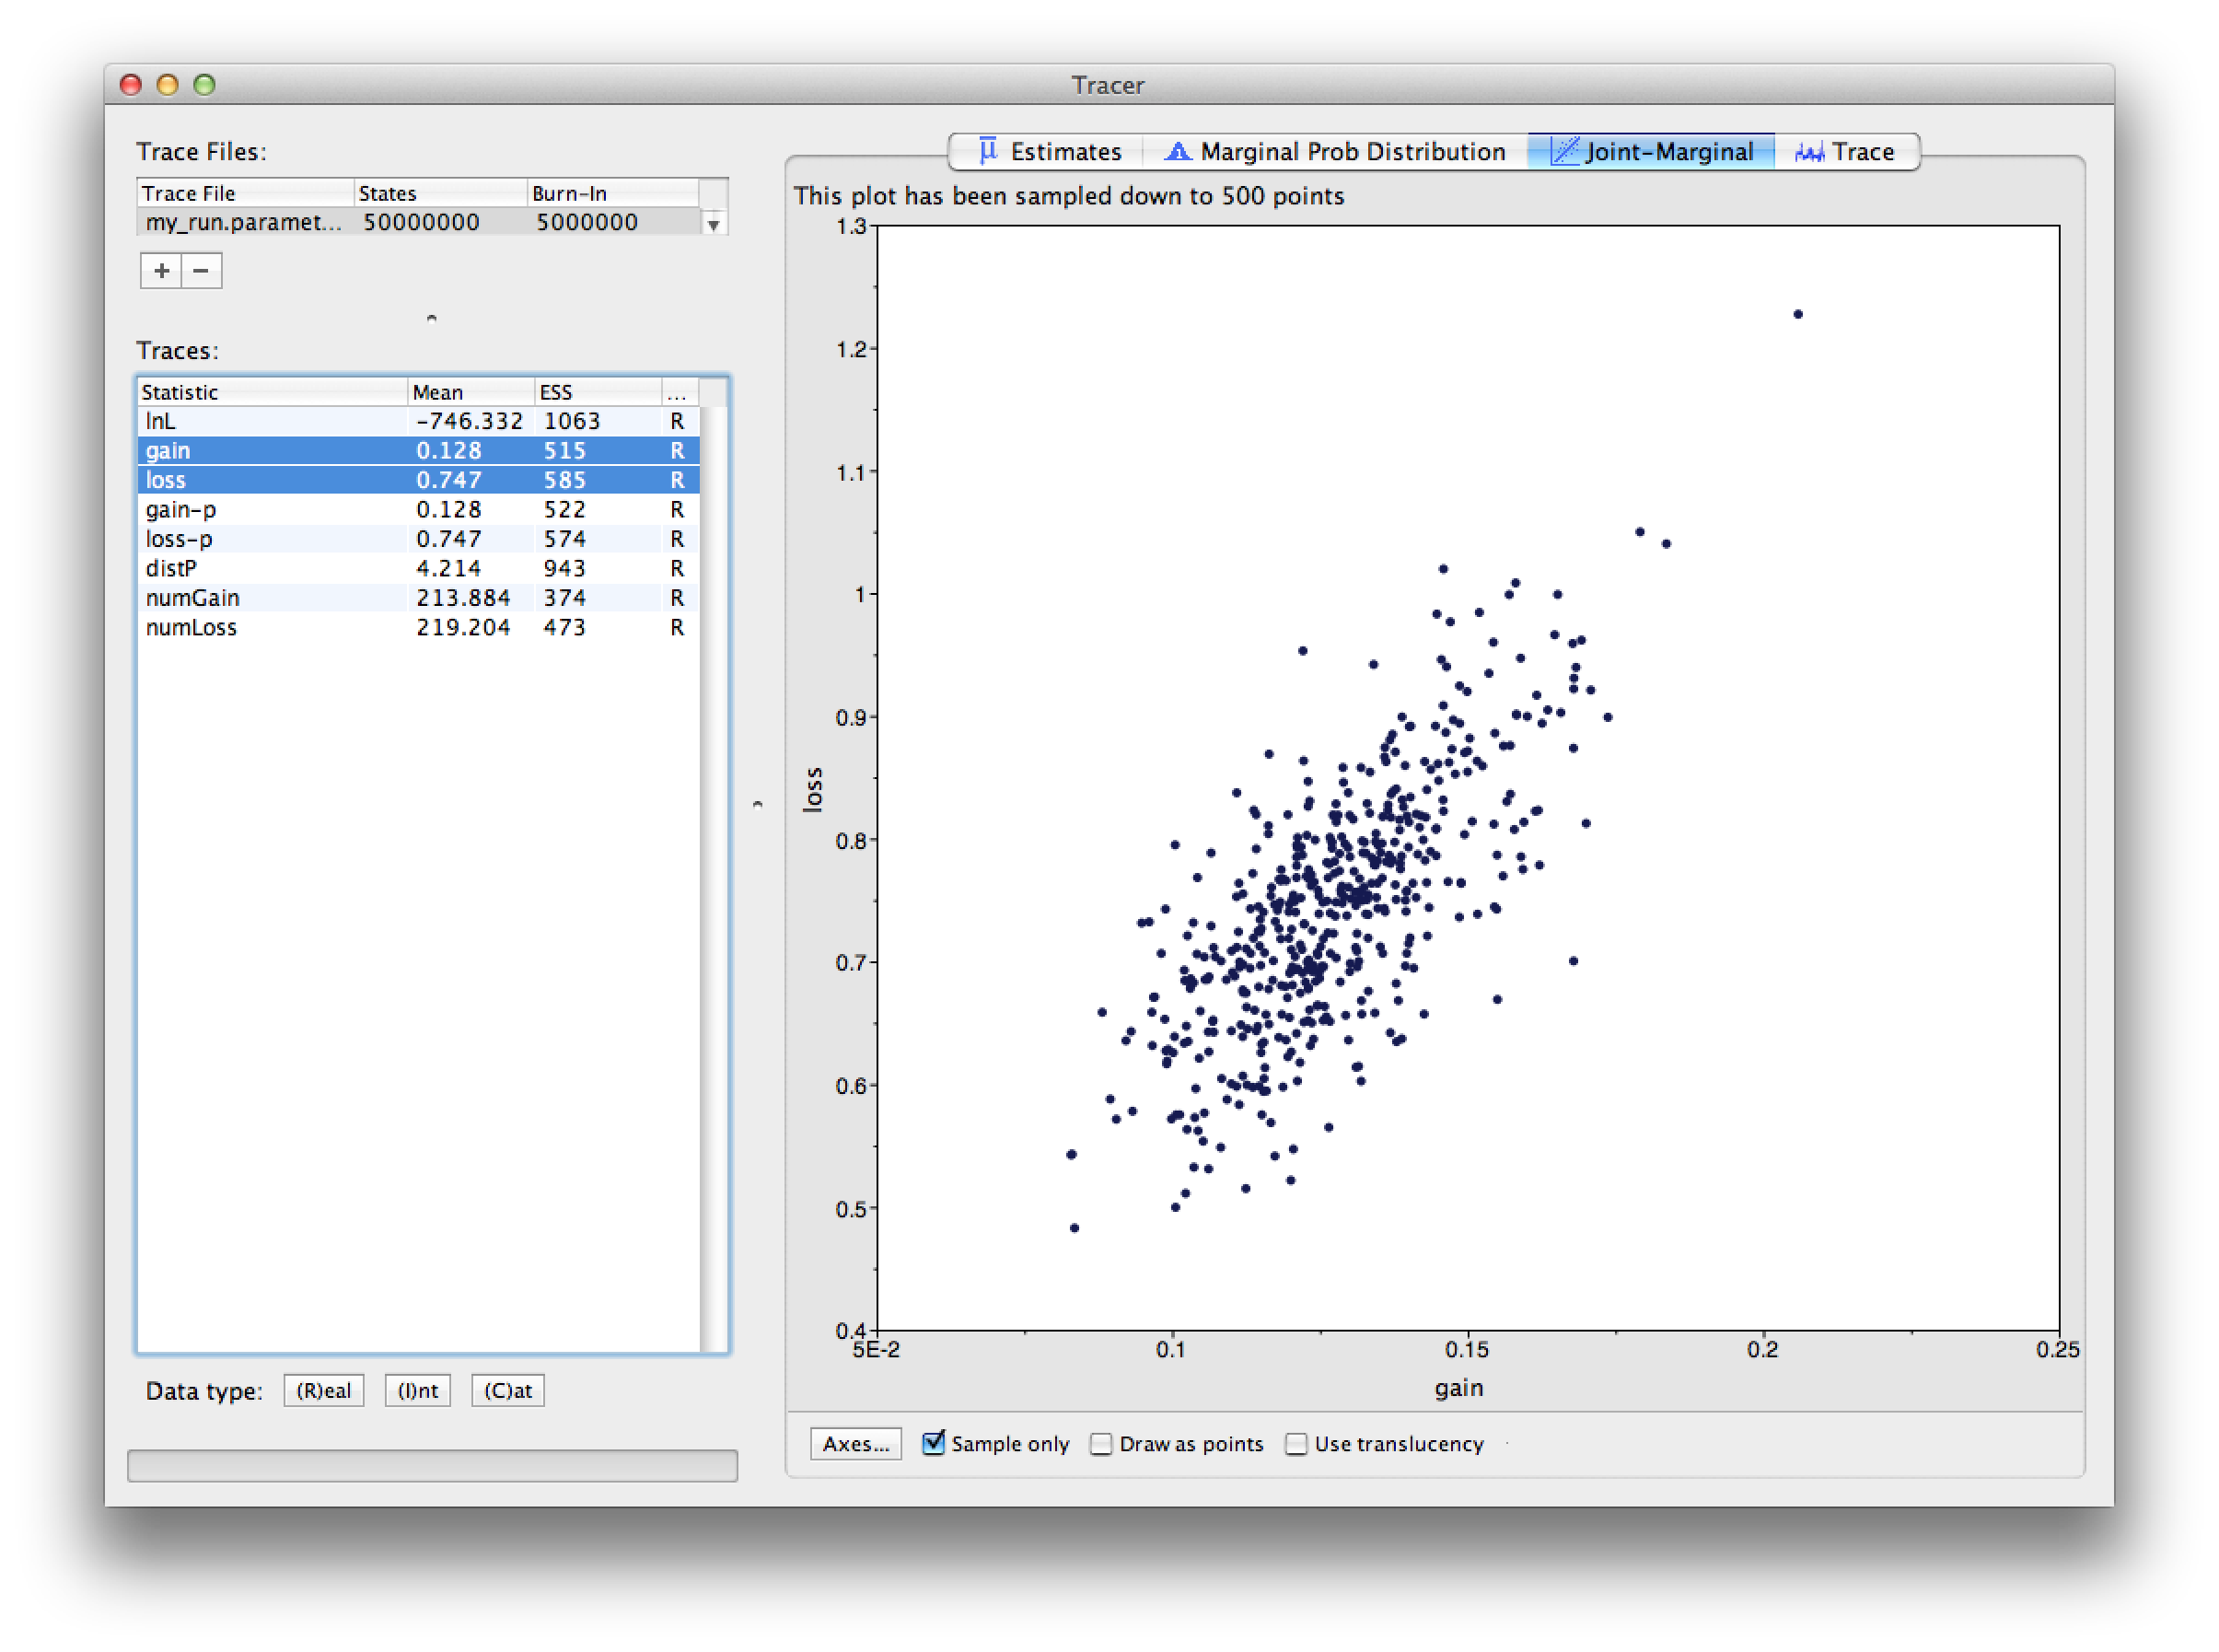
\includegraphics[width=2.5in]{figures/loss_gain}
%\end{figure}
%
%The Joint-Marginal of rate of area gain and loss parameters shows strong positive correlation.
%This correlation arises partly because the proportion of occupied areas is greatly influenced by the ratio of rate of area gain to rate of area loss.
%For example, when the rates of area gain and loss are equal, range sizes tend to equal half the total number of areas.
%
%\noindent \\ \impmark Highlight the ``loss'' and ``numLoss'' parameters then click Joint-Marginal. Do the same for ``gain'' and ``numGain''. \\
%
%\begin{figure}[H]
%\centering
%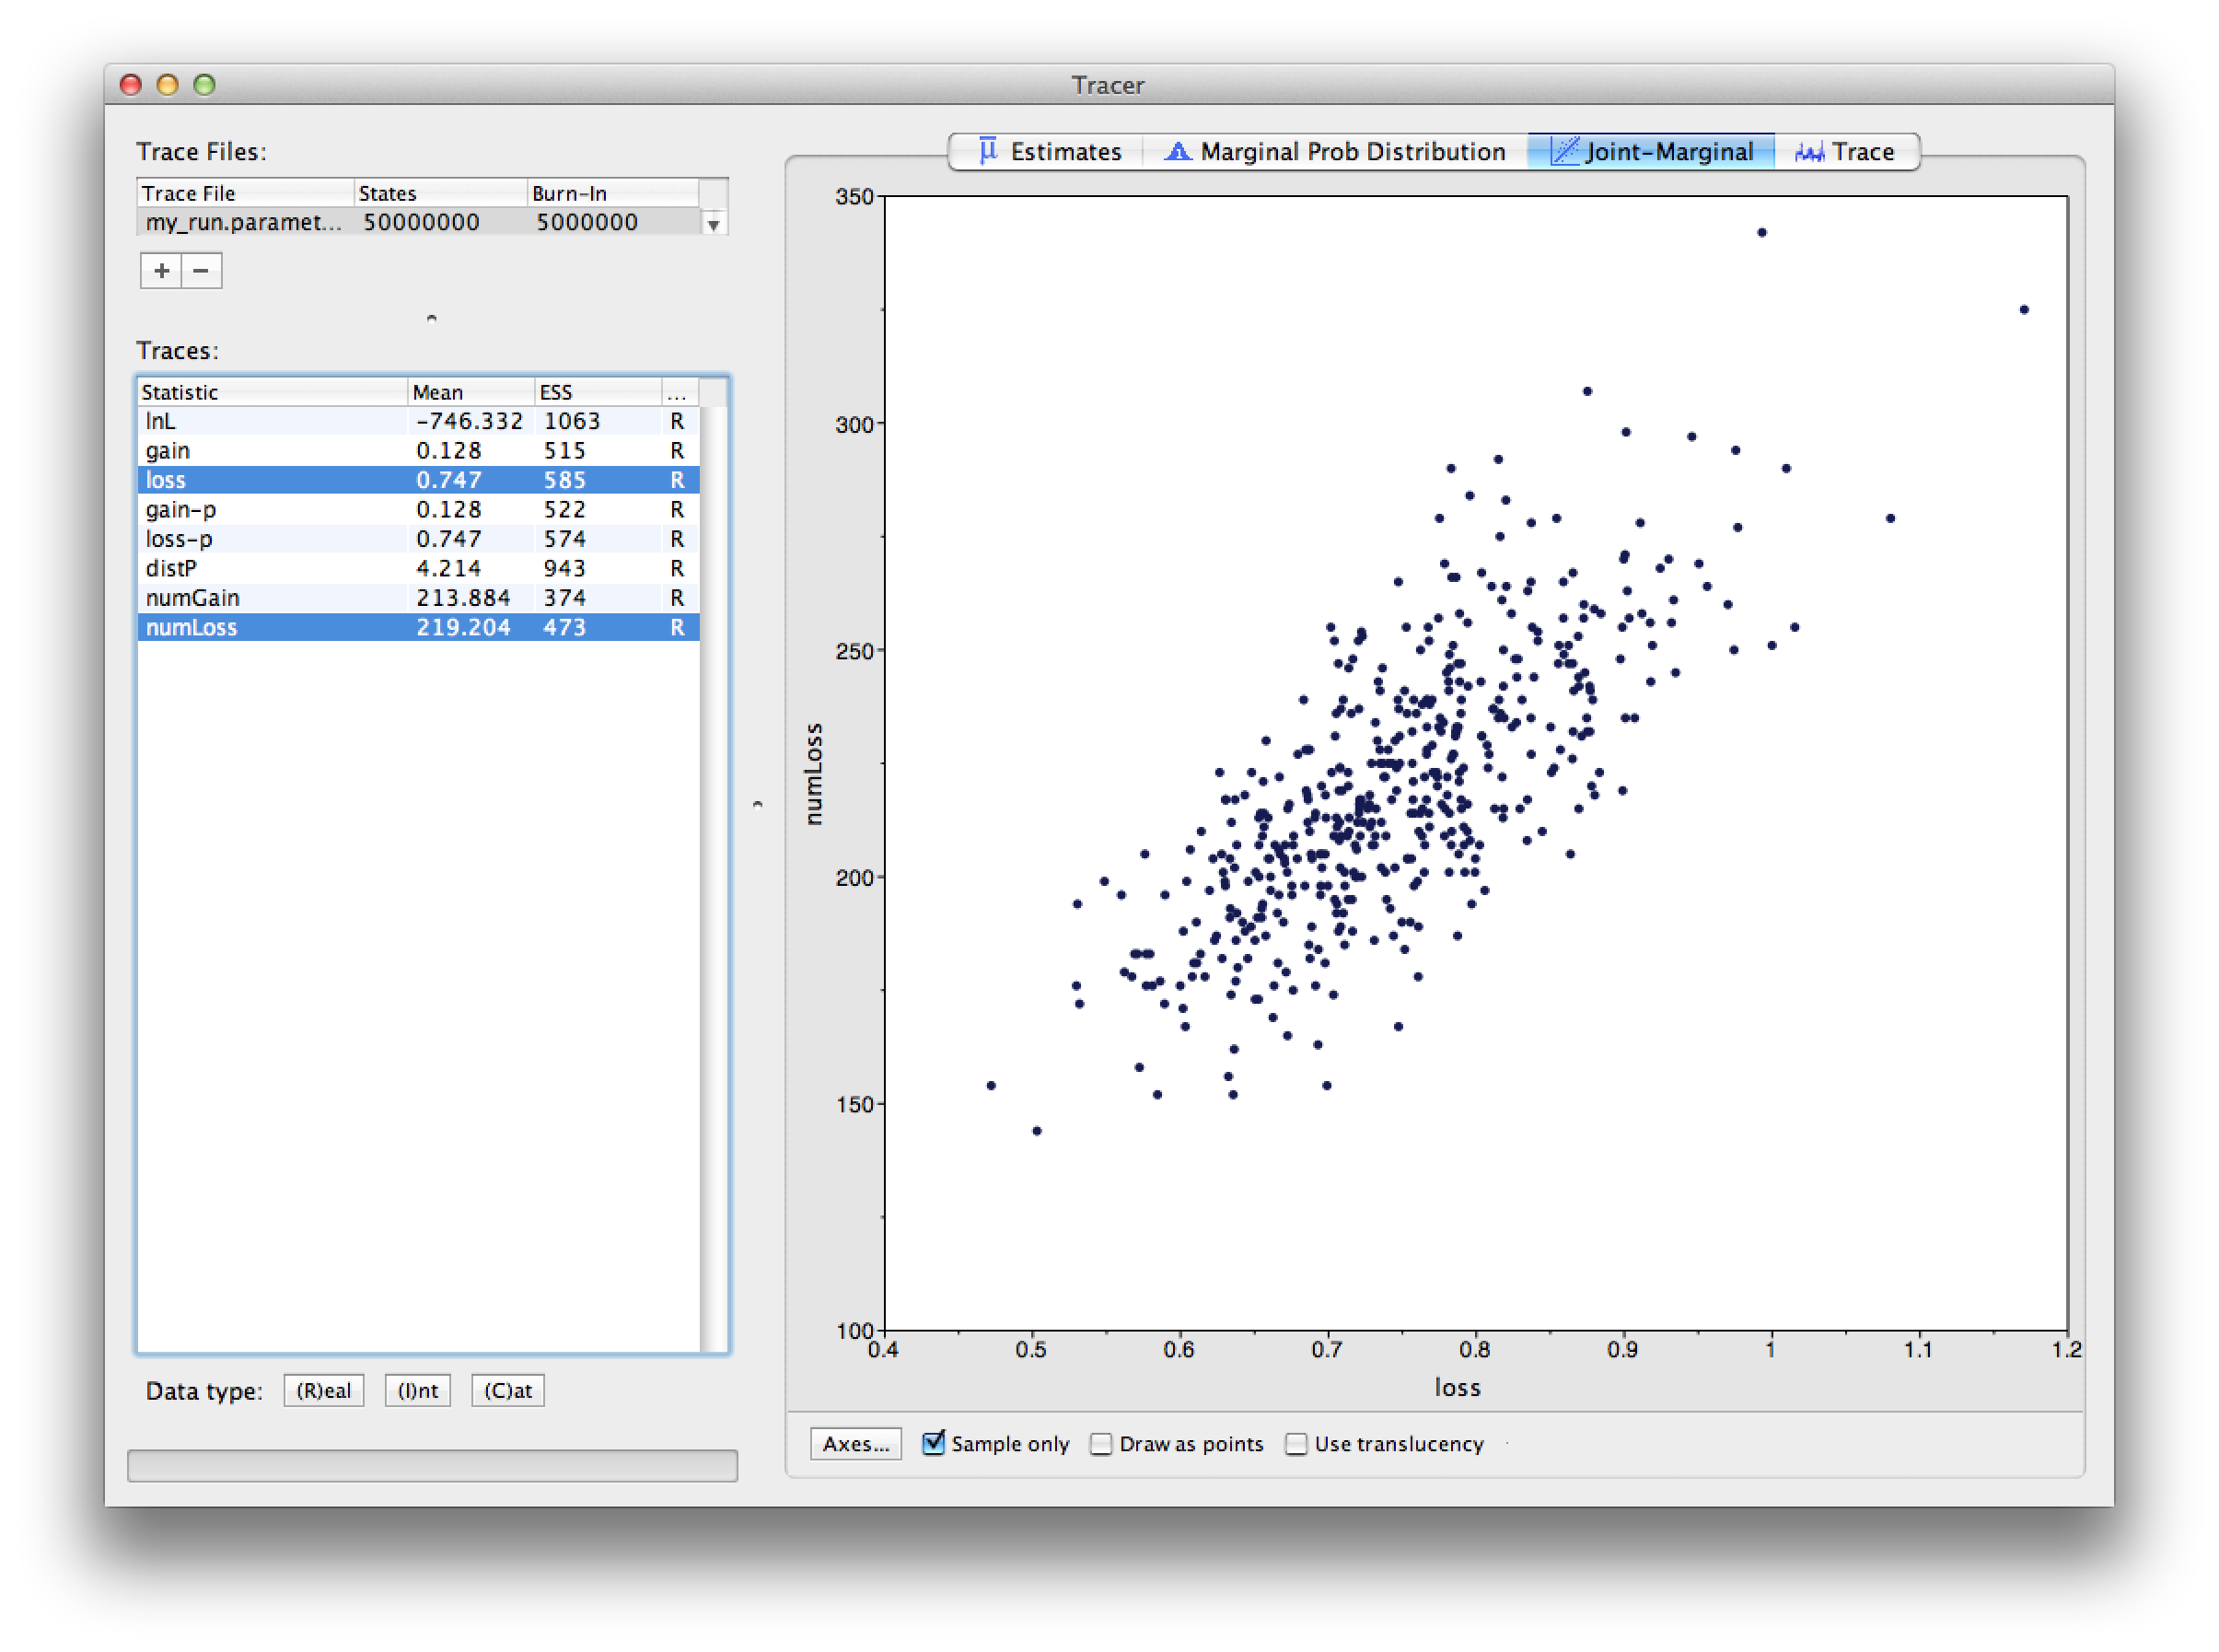
\includegraphics[width=2.5in]{figures/loss_numloss}
%\end{figure}
%
%Again, we see strong positive correlation.
%This is reassuring, since we expect to see many sampled range gain and loss events when the corresponding rates are high.
%
%\noindent \\ \impmark  Highlight the ``gain'' and ``distP'' parameters then click Joint-Marginal. Do the same for ``loss'' and ``distP''.\\
%
%\begin{figure}[H]
%\centering
%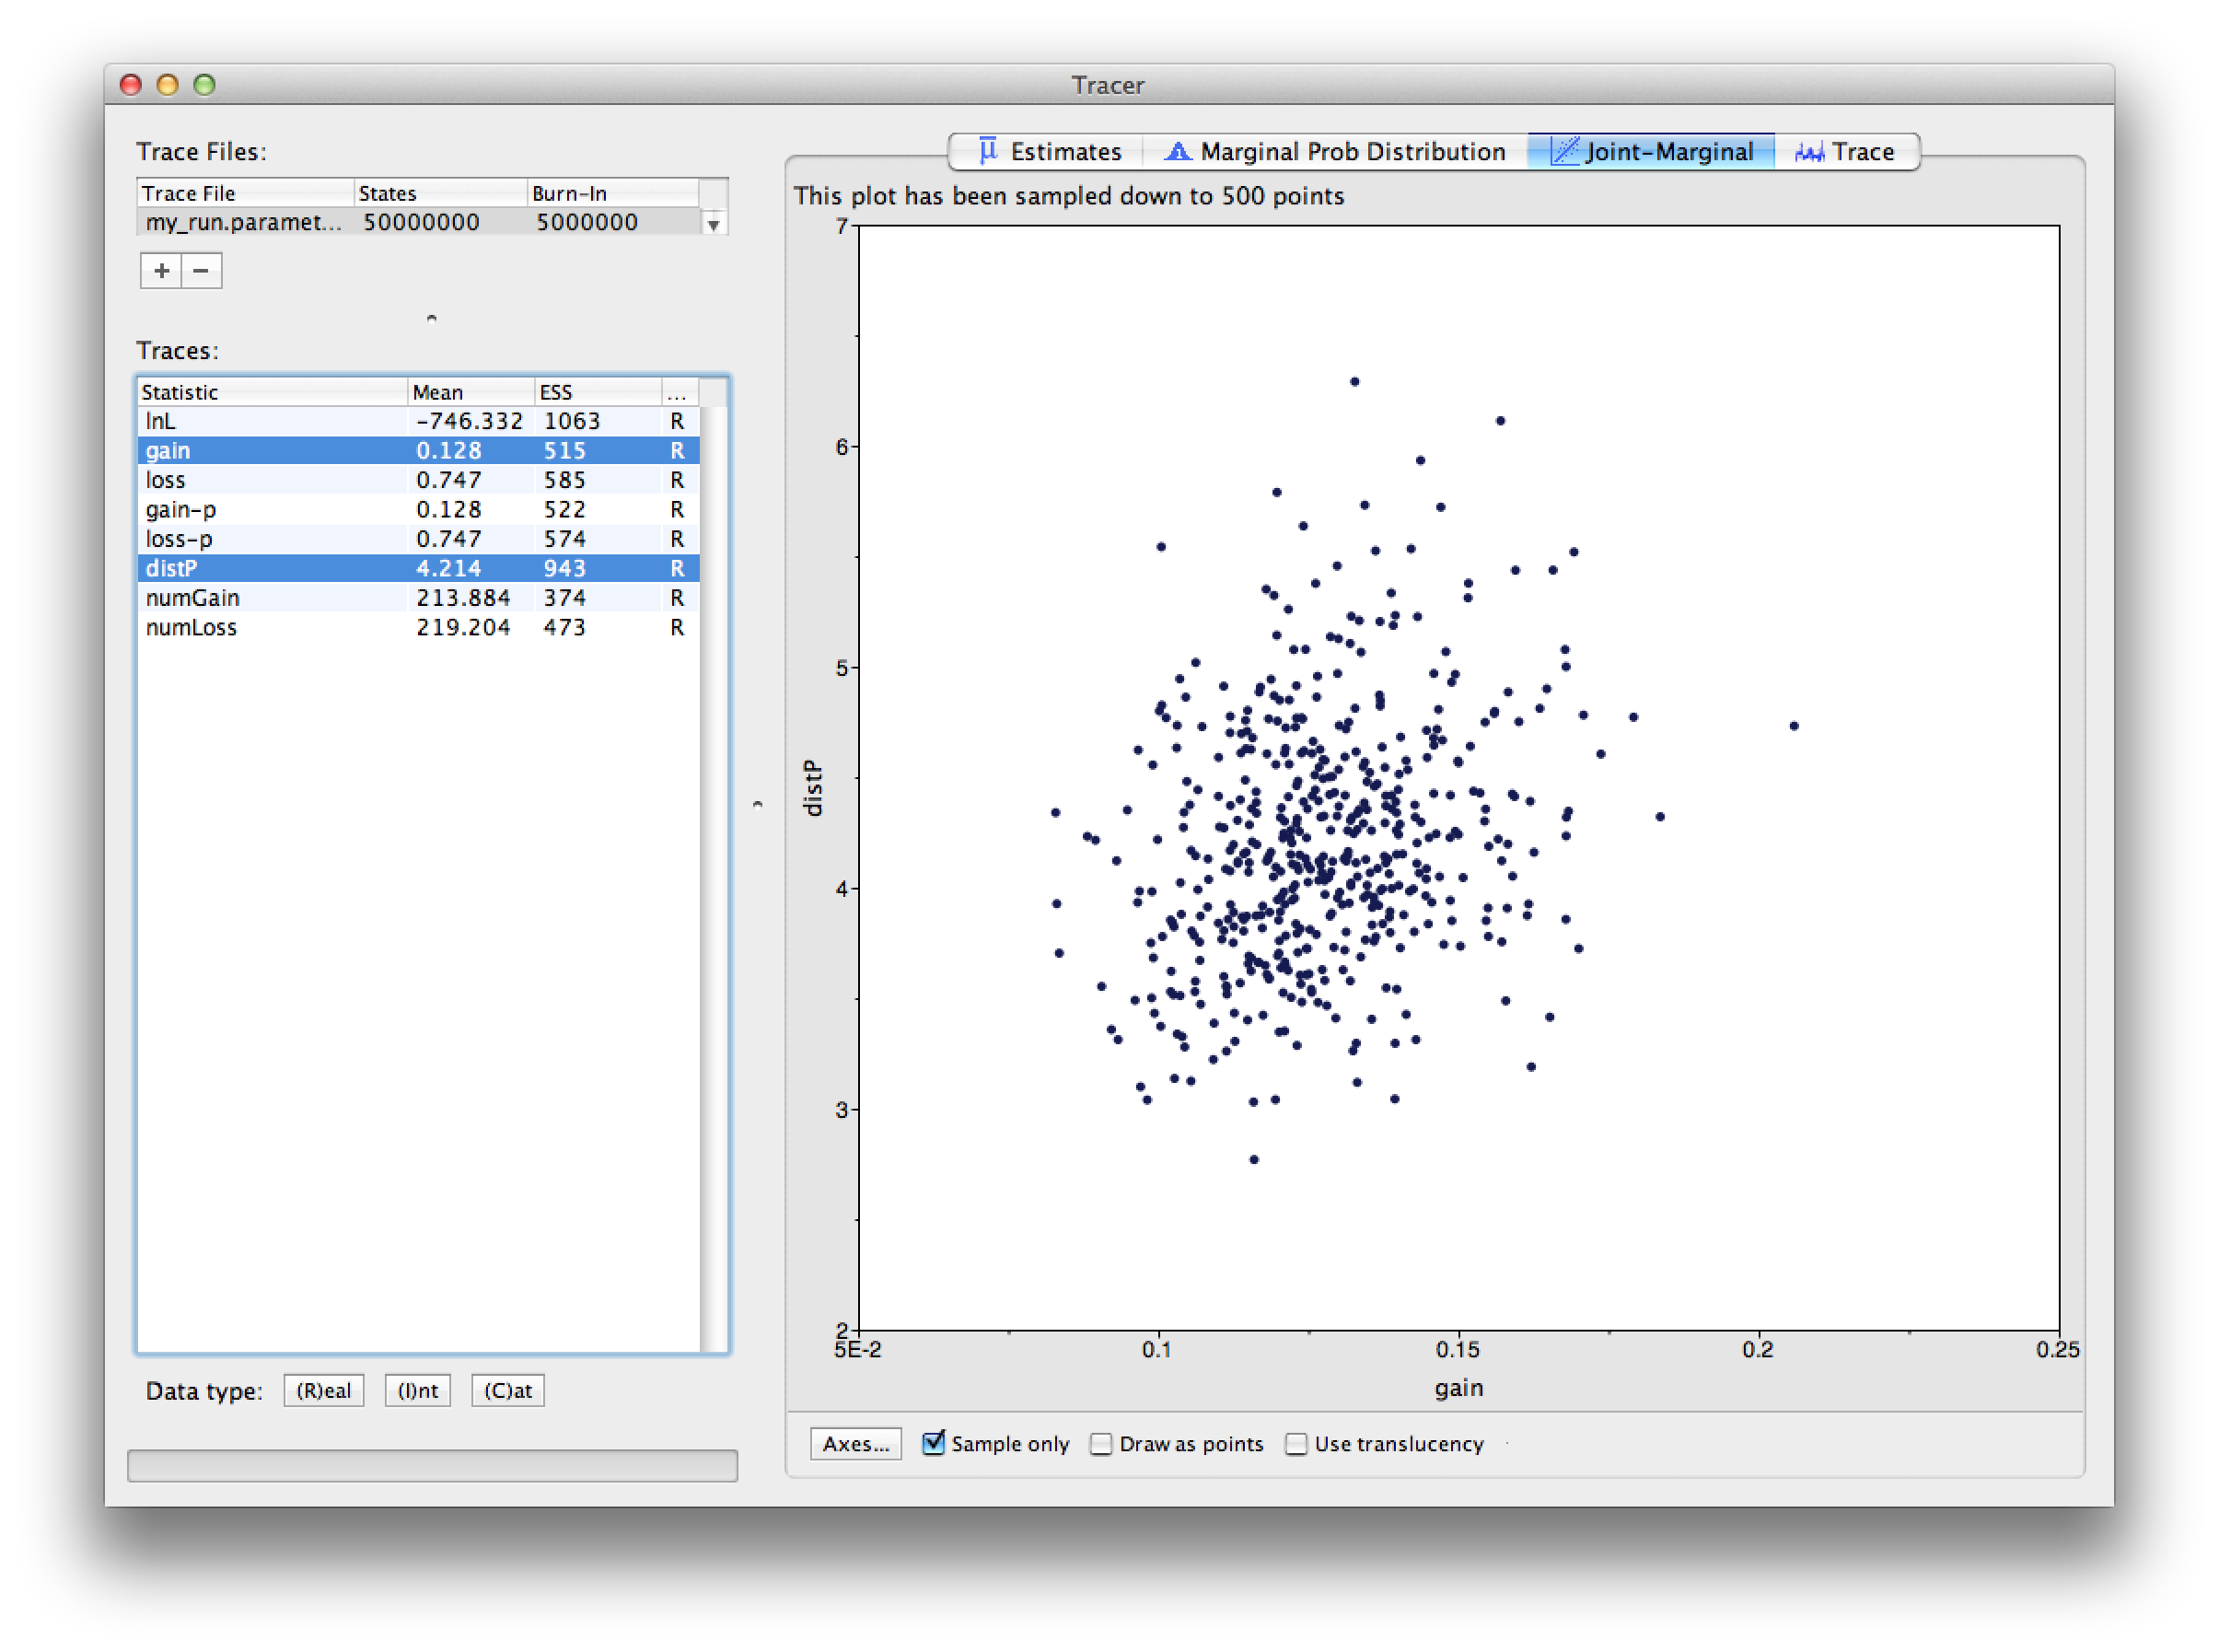
\includegraphics[width=2.5in]{figures/gain_distp}
%\end{figure}
%
%For the simulated data we don't see any strong correlation between either rate of loss or gain and the distance power parameter, but this is not always the case.
%Large distance power parameters sometimes results in rates of area gain and loss being underestimated in value, resulting in a mild negative correlation.
%
%\noindent \\ \impmark Highlight all parameters and click Estimates.
%
%\begin{figure}[H]
%\centering
%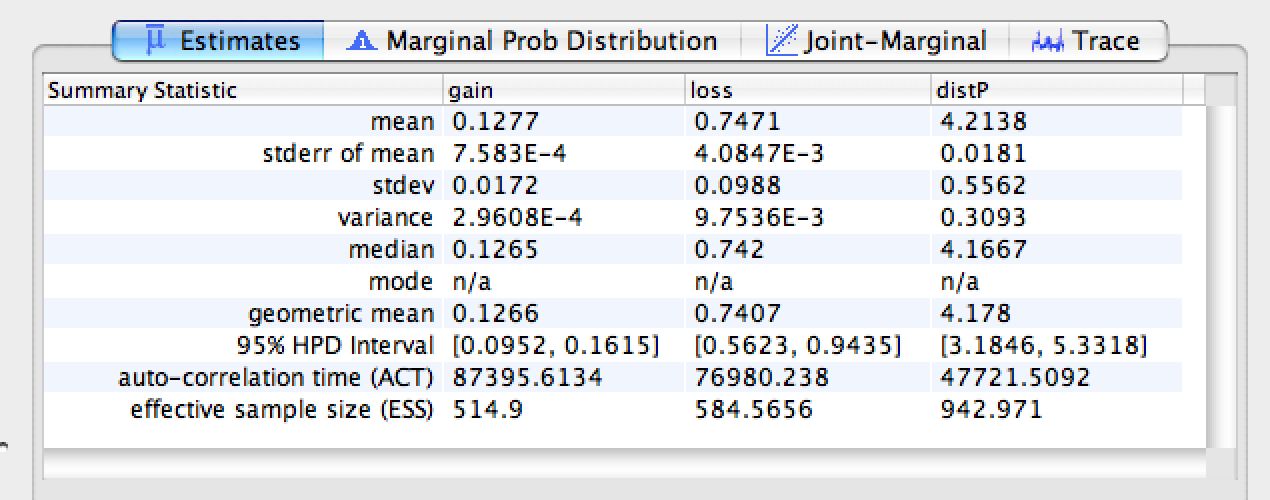
\includegraphics[width=2.5in]{figures/hpd}
%\end{figure}
%
%This gives you a handy selection of summary statistics.
%Of course we typically don't know the true parameter values, but we should be reassured to learn the true parameter values for gain, loss, and distP (0.1, 0.7, and 4.0, respectively) reside within their corresponding 95\% HPD Intervals.
%It's also interesting to note that the distance power parameter has a much wider interval that the rate parameters, suggesting there is less information in the data for this parameter.
%


%The Gelman-Rubin convergence diagnostic tests whether two MCMC analyses converged to the same distribution (e.g. the posterior).
%It does this by computing potential scale reduction factors (PSRFs) for all parameters, which compares the within-chain parameter variance to the between-chain parameter variance.
%There's no hard rule, but PSRF values close to 1.0 show convergence while PSRF values greater than 1.1 raise concern.
%Below, we can quickly compute the PSRFs for \texttt{my\_run.parameters.txt} and \texttt{my\_other\_run.parameters.txt} using the R package, coda.
%
%\noindent \\ \impmark Open the R console and enter the following commands.
%\begin{framed}
%\begin{lstlisting}
%> install.packages('coda')
%...
%> library('coda')
%> run1 = mcmc(read.table('my_run.parameters.txt',header=T))
%> run2 = mcmc(read.table('my_other_run.parameters.txt',header=T))
%> gelman.diag(mcmc.list(run1,run2))
%>
%Potential scale reduction factors:
%
%        Point est. Upper C.I.
%n              NaN        NaN
%lnL           1.00       1.00
%gain          1.01       1.01
%loss          1.00       1.01
%gain.p        1.00       1.01
%loss.p        1.00       1.01
%distP         1.00       1.00
%numGain       1.01       1.02
%numLoss       1.00       1.01
%
%Multivariate psrf
%
%1
%\end{listing}
%\end{framed}

%\subsection{Sampled range histories (\texttt{my\_run.area\_states.txt})}
%
%This file reports the stochastically mapped range histories sampled every \texttt{historySampleFrequency} iterations.
%From this we can compute the {\it marginal} posterior probability of any given area being occupied simply by finding the frequency the area was marked present (1), which we'll call the {\it marginal area posterior probability}.
%You may be interested in not only the marginal posterior of area occupancy, but the marginal posterior of the joint distribution of areas, which we'll call the {\it marginal range posterior probability}.
%For example, say your range contains 4 areas, and taxon A is present only in areas 1 and 2 for half of all MCMC samples and only present in areas 3 and 4 for the remaining half.
%The marginal area posterior range would report a 0.5 probability of any given area being occupied.
%The marginal range posterior would give you richer information, that the range was either composed of areas 1 and 2 or of 3 and 4, but never 1 and 3, 1 and 4, 2 and 3, or 2 and 4.
%
%Here we will use Python to report the marginal range probability for the range belonging to the most recent common ancestor (MRCA) shared by the species named \texttt{t1} and \texttt{t2} ordered by their posterior probabilities. We'll call this node MRCA(t1,t5).
%
%\noindent \\ \impmark Change directories to \texttt{examples}.
%
%\begin{framed}
%\begin{lstlisting}
%> cd examples
%\end{lstlisting}
%\end{framed}
%
%\noindent \\ \impmark Open the Python console and enter the following commands.
%
%\begin{framed}
%\begin{lstlisting}
%>>> from pp_range import *
%>>> range_dict = make_range_dict('my_run.area_states.txt', fburn=0.25)
%>>> area_coords = get_area_coords('my_geo.txt')
%>>> idx_list = get_node_idx_list('my_run.area_states.txt')
%>>> node_key = get_node_key('my_tree.txt', 't1', 't5', idx_list)
%>>> best_ranges = get_best_ranges(range_dict, node_key)
%>>> prob_area_pairs = make_posterior_area_pairs(range_dict, node_key)
%>>> best_area_pairs = get_best_area_pairs(prob_area_pairs)
%>>> best_areas = get_best_area_pairs(prob_area_pairs, show_marginal=True)
%\end{lstlisting}
%\end{framed}
%
%\noindent \\ \impmark To list the five most probable ranges for MRCA(t1,t5), type
%\begin{framed}
%\begin{lstlisting}
%>>> best_ranges[0:5]
%[('000000000000000000000000001111000', 0.022660623833644103),
% ('000000000000000000000000001011000', 0.01759530791788836),
% ('000000000000000000000000011111000', 0.01652892561983452),
% ('000000000000000000000000011011000', 0.0146627565982403),
% ('000000000000000000010000001111000', 0.01226339642761916)]
%
%>>> sum([p[1] for p in best_ranges[0:5]])
%0.08371101039722645
%\end{lstlisting}
%\end{framed}
%
%The second column gives the probability of the entire MRCA(t1,t5) range shown in the first column.
%There's a fair deal of uncertainty the MRCA(t1,t5) range reconstruction, since these best five ranges only account for about 0.08 of the probability.
%
%\noindent \\ \impmark To list the five most probable area co-occurrences in the MRCA(t1,t5) range, type
%\begin{framed}
%\begin{lstlisting}
%>>> best_area_pairs[0:5]
%[((26, 29), 0.60650493201812505),
% ((26, 28), 0.57717941882164425),
% ((28, 29), 0.54385497200746136),
% ((26, 27), 0.42282058117834981),
% ((27, 28), 0.41242335377232475)]
% 
%>>> best_areas[0:5]
%[((26, 26), 0.78459077579311998),
% ((29, 29), 0.77179418821647394),
% ((28, 28), 0.74193548387096575),
% ((26, 29), 0.60650493201812505),
% ((26, 28), 0.57717941882164425)]
%
%\end{lstlisting}
%\end{framed}
%
%Note the values in \texttt{best\_areas} are the marginal area probabilities.
%These correspond to the diagonal entries in the heatmap below and to the values in \texttt{my\_run.area\_probs.txt} and \texttt{my\_run.nhx}.
%
%\noindent \\ \impmark To visualize these probabilities as a heatmap, type
%\begin{framed}
%\begin{lstlisting}
%>>> title_str = 'Prob(areas i,j co-occur in MRCA(t1,t5) range)'
%>>> plot_posterior_area_pair(prob_area_pairs, title_str)
%\end{lstlisting}
%\end{framed}
%
%\begin{figure}[H]
%\centering
%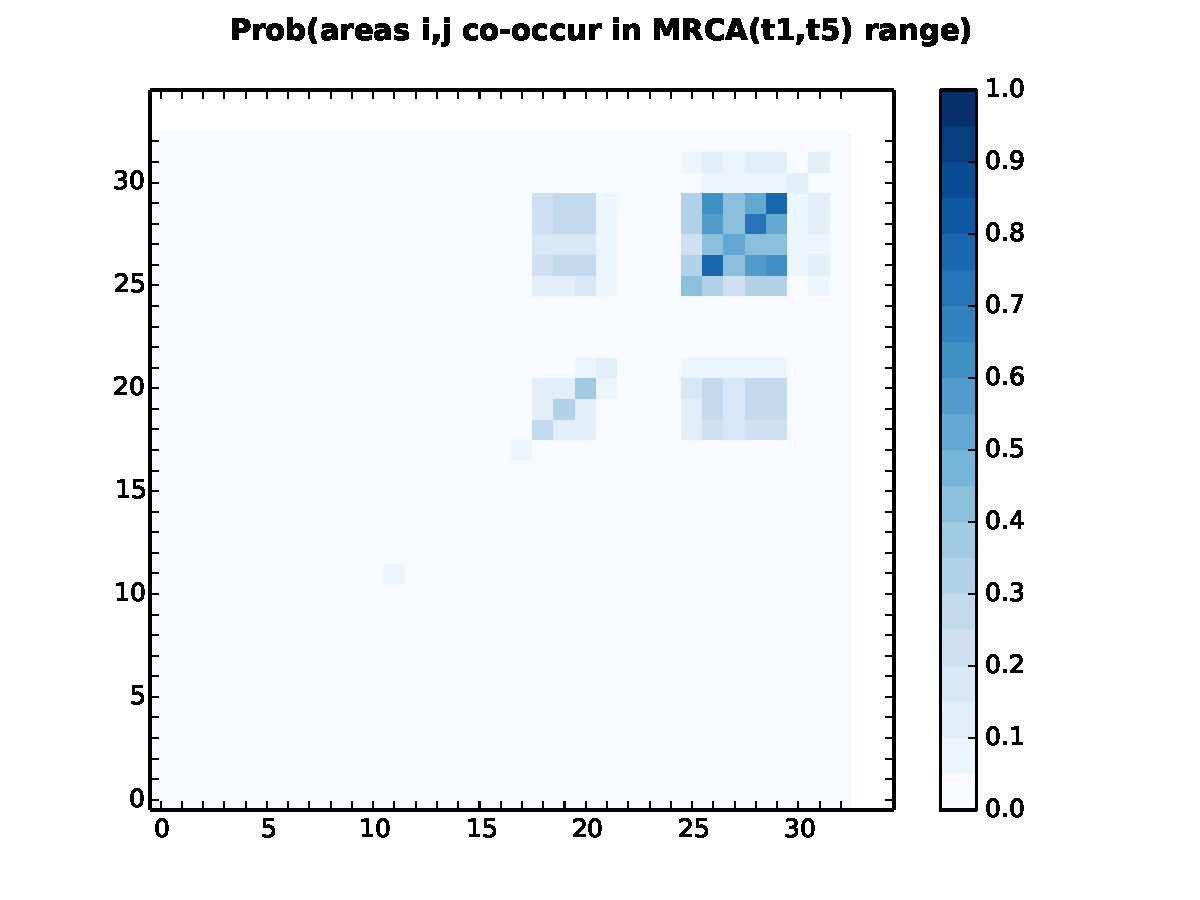
\includegraphics[width=4in]{figures/range_area_pair_pp}
%\end{figure}
%
%As indicated from the list produced by \texttt{get\_best\_area\_pairs()}, we see the inference gives moderate support for areas 26, 28, and 29 being co-occupied by MRCA(t1,t5).
%Referring to \texttt{my\_geo.txt}, we see these areas are geographically close and located in south-eastern Australia.
%You can also retrieve the coordinates through the \texttt{area\_coords} dictionary.
%
%\noindent \\ \impmark To query the geographical coordinates for an area, type
%\begin{framed}
%\begin{lstlisting}
%>>> area_coords[26]
%{'lat': -32.5, 'lon': 137.5}
%
%>>> area_coords[28]
%{'lat': -32.5, 'lon': 147.5}
%
%>>> area_coords[29]
%{'lat': -32.5, 'lon': 152.5}
%\end{lstlisting}
%\end{framed}
%
%\subsection{Posterior probabilities of range histories (\texttt{my\_run.area\_probs.txt})}
%
%Each row of this tab-delimited file contains information about that node's range.
%The rows are ordered in postorder traversal (aka pruningwise).
%The first column gives the taxon name.
%The remaining columns correspond to areas, maintaining the same order as all other files (e.g. the second column is the first area, the $n$th column is the ($n-1$)th area).
%These entries report the marginal area probability of the taxon (row) occupying the area (column).
%These probabilities are computed the frequency that the area was marked present from the data contained in \texttt{my\_run.area\_probs.txt}, a quantity that cannot be computed until the MCMC analysis completes.
%Because MCMC does not accurately sample from posterior during burn-in, some number of initial cycles are discarded as specified by the \texttt{probBurnIn} flag.